\chapter{实验与验证}

本章介绍了\toolname{}的实验。
围绕五个研究问题,设计实验,根据结果回答了五个研究问题。

\section{研究问题}

本文提出了一个结合了基于频谱的缺陷定位和基于状态覆盖的缺陷定位的缺陷定位框架,
并且通过结合深入分析基于频谱的缺陷定位和基于状态覆盖的缺陷定位能够准确定位的原因。
本文还使用了机器学习方法去预测谓词,探讨了谓词类型在缺陷定位中的作用。

本文试图回答以下几个问题:
\begin{enumerate}
\item \textbf{当使用不同的数据收集粒度时,缺陷定位技术的效果有什么不同?} \\
这个研究问题探索了数据收集的粒度对缺陷定位结果的影响。
最近研究使用的方法级别的缺陷定位从两个维度收集数据:
语句级别和方法级别。
但是没有现有方法探究了数据收集粒度对缺陷定位结果的影响。
因为从不同的粒度收集数据会导致谓词数量的不同,
而谓词数量对执行时间影响程度也不清楚。
\item \textbf{不同的怀疑度计算公式会如何影响缺陷定位的结果?} \\
这个研究问题探索了缺陷定位公式的重要性,
并分析了是否还能通过改进缺陷定位公式去提升缺陷定位效果,
为后续研究提供了参考。
\item \textbf{缺陷定位技术的不同结合方式效果如何?} \\
在章\ref{sec:approach_comb}中,
本文探讨了结合缺陷定位技术的方法。
这个研究问题研究了不同结合方式的效果。
\item \textbf{机器学习模型预测谓词的准确率如何?} \\
这个研究问题探索了谓词预测模型的准确率,
并且在不同的机器学习模型上进行了对比。
\item \textbf{哪种谓词能够更好地帮助定位?} \\
这个研究问题比较了基于谓词预测的缺陷定位和本文提出的结合方法、现有方法之间的结果,
分析谓词在定位缺陷中的作用和不足。
% \item \textbf{和现有很多缺陷定位方法相比,本文的方法效果如何?} \\

\end{enumerate}

\section{实验数据}

本文使用Defects4j数据集\parencite{Just2014Defects4J}(v1.0)作为实验对象,
下文所提到的Defects4j都是 v1.0 版本。
Defects4j数据集含有357个真实的缺陷,来自五个大型的开源软件项目,见表\ref{defects4j_details}。
其中,“实验缺陷数目”是本文在实验中实际使用了的缺陷数目,“代码行数(千行)”表示的是这五个项目最近的版本的代码行数。
本文只使用了330个缺陷是因为其余27个缺陷因为插装后的代码太大导致“code too large"的报错而无法运行。

\begin{table}
\centering
\begin{tabular}{|l|r|r|r|r|}
\hline
项目名称 & 缺陷数目 & 实验缺陷数目 & 代码行数(千行) & 测试用例数目 \\
\hline
JFree\textbf{Chart} & 26 & 26 & 96 & 2205 \\
\hline
\textbf{Closure} compiler & 133 & 122 & 90 & 7927 \\
\hline
Apache commons-\textbf{Math} & 106 & 98 & 85 & 3602 \\
\hline
Apache commons-\textbf{Lang} & 65 & 57 & 22 & 2245 \\
\hline
Joda-\textbf{Time} & 27 & 27 & 28 & 4130 \\
\hline
总计 & 357 & 330 & 321 & 20109 \\
\hline
\end{tabular}
\caption{Defects4j数据集缺陷情况}
\label{defects4j_details}
\end{table}

\section{实验标准}

为了验证本文提出的结合后的缺陷定位的效果,以及预测谓词的效果,
需要一套衡量缺陷定位效果的标准和预测谓词效果的标准。

\subsection{缺陷定位结果标准}

本文使用两种常用的缺陷定位标准: Top-k 的召回率和 EXAM 分数。

Top-k 的召回率衡量的是有多少缺陷能够排在怀疑列表的前k位。
根据Kochhar等人的研究\parencite{Kochhar2016Practitioners},
超过73\%的参与者认为观察怀疑列表的前5个程序元素是可以接受的,
几乎所有参与者都认为10个程序元素是可以接受的最大的需要观察的程序元素个数。
所以本文采用1,3,5,10作为k值。
对于怀疑度分数相同的程序元素,它们的排名会使用平均排名,这也是很多已有研究使用的方法\parencite{Pearson2017Evaluating,Xuan2014Learning,Steimann2013Threats,Wong2016A}。

EXAM 分数衡量的是开发者需要查看多少个位置才能看到真正的缺陷。
$$
\mathrm{EXAM} = \frac{n}{N}
$$
其中$N$表示候选的程序元素个数(比如被失败的测试用例覆盖的语句),$n$表示缺陷程序元素排在怀疑度列表的第$n$位。
EXAM 分数是一个0到1之间的值,且值越小越好。
它反映出了含有缺陷的程序元素在所有可疑程序元素中的相对位置,
体现出整个缺陷定位方法的效果。
很多工作都使用了这个方法\parencite{Wong2012Effective,Pearson2017Evaluating}。

\subsection{谓词预测结果标准}

本文对谓词预测结果的评判方法采用机器学习分类问题的评判方法。

首先引入一些评估分类问题效果时需要的统计量。
混淆矩阵统计量见表\ref{confusion_matrix}。
样本总数为$N$。
正例反例为两个相对的概念。
对于多分类问题,其余分类都为反例。

\begin{table}
\centering
\begin{tabular}{|c|c|c|}
\hline
\multirow{2}*{真实情况} & \multicolumn{2}{c|}{预测结果} \\
\cline{2-3}
~ & 正例 & 反例 \\
\hline
正例 & TP(真正例) & FN(假反例) \\
\hline
反例 & FP(假正例) & TN(真反例) \\
\hline
\end{tabular}
\caption{分类结果混淆矩阵}
\label{confusion_matrix}
\end{table}

准确率(accuracy)衡量的是分类正确的样本数占样本总数的比例:
$$
\mathrm{Accuracy} = \frac{TP + TN}{N} = \frac{TP + TN}{TP + FN + FP + TN}
$$
。

准确率能够衡量一个机器学习模型的预测情况,但是有的时候只有准确率还不够。
有的时候人们还关心查准率和召回率。

查准率(precision)衡量的是被分类为正例的样本中有多少是真的正例:
$$
\mathrm{Precision} = \frac{TP}{TP + FP}
$$。

查全率或召回率(recall)衡量的是正例中有多少被分类为正例:
$$
\mathrm{Recall} = \frac{TP}{TP + FN}
$$。

查准率和查全率是一对相互矛盾的度量。
一般来说,查准率高时,查全率低,而查准率低时,查全率高。
F1 度量结合查准率和查全率,给出一个便于比较的统一的值:
$$
\mathrm{F1} = \frac{2 \times \mathrm{Precision} \times \mathrm{Recall}}{\mathrm{Precision} + \mathrm{Recall}}
$$。

对于二分类问题来说,正例负例就是二分类的两个类别。
但是对于多分类来说,每个类都可以是正例,这时其余类别就是负例。
所以多分类问题的查准率,查全率和 F1 的对数和分类的类别数量一致。
如果分类的类别数量非常多,观察庞大的查准率、查全率和 F1 并不能直观地描述预测结果,
需要将各个分类的查准率、查全率和 F1 结合起来。
$TP_i,FN_i,FP_i,TN_i$表示多分类问题下,分类$i$的真正例、假反例、假正例和真反例的数目。
分类数记为$C$,$c_i$表示分类为$i$的样本数量。
多分类问题的查准率、查全率和 F1 有以下几种结合方式:
\begin{itemize}
\item \textbf{micro}:\\
先在全局的角度计算真正例、假反例和假正例的个数,然后带入公式计算查准率、查全率和 F1。
以查准率为例:
$$
\mathrm{Precision} = \frac{\sum_{i=1}^C{TP_i}}{\sum_{i=1}^C{(TP_i + FP_i)}}
$$。
\item \textbf{macro}:\\
先收集每个分类的真正例、假反例和假正例的个数,带入公式计算每个分类的查准率、查全率和 F1,最后求均值。
这个不会考虑标签的不均衡。
以查准率为例:
$$
\mathrm{Precision_i} = \frac{TP_i}{TP_i + FP_i}
$$
$$
\mathrm{Precision} = \frac{1}{C}\sum_{i=1}^c{\mathrm{Precision_i}}
$$。
\item \textbf{weighted}:\\
先收集每个分类的真正例、假反例和假正例的个数,带入公式计算每个分类的查准率、查全率和 F1,最后根据
分类的支持度(该分类的样本在总样本中所占的数目)分配权重求均值。
这个算法与 macro 相比,考虑了标签的不均衡性。
以查准率为例:
$$
\mathrm{Precision_i} = \frac{TP_i}{TP_i + FP_i}
$$
$$
\mathrm{Precision} = \sum_{i=1}^c{\frac{c_i}{C}\mathrm{Precision_i}}
$$。
\end{itemize}

本文采用weighted的方式得到多分类问题的查准率、查全率和F1。

\section{实验设置}

\subsection{数据收集粒度}

本文考虑两种数据收集粒度:语句级别和函数级别。
因为本文关注于函数的缺陷定位,所以对于函数级别的数据收集,
只需要直接在函数的出入口收集就可以。
而对于语句级别的数据收集,则需要取一个函数内所有语句的最大怀疑度值作为这个函数的怀疑度。
本文默认配置使用语句级别的数据收集。

\subsection{怀疑度公式}
\label{sec:exp_all_formula}

怀疑度的公式上,本文实现了七种怀疑度计算的公式。
五种是经典的基于频谱的缺陷定位公式见表\ref{susp_formula},
两种是基于频谱的缺陷定位的公式\ref{eq:sd}和公式\ref{eq:sober}。
本文默认配置使用Ochiai作为怀疑度公式。

\subsection{结合怀疑度的方法}

在章\ref{sec:approach_comb}的讨论中,
本文使用了公式
$$
c(s,e,r) = max_{p \in s(e)}r(p)
$$
计算得到了程序元素$e$的怀疑度,
并提出了\textsc{MaxPred}和\textsc{LinPred}两种结合方式。

在本文的实验中,默认配置使用$\alpha = 0.5$的\textsc{LinPred}。
其中,第一个怀疑度使用基于频谱的缺陷定位计算得到($s_0(e)$产生的谓词恒为\mycode{true}),
第二个使用预定义或预测谓词频谱信息计算得到。

\subsection{谓词}

为了探索谓词在缺陷定位中的作用,本文把谓词分为三大类:预定义谓词、预测谓词和恒真谓词。
对预定义谓词,又根据其定义分为三类:分支、返回和数值对。
在本文的实验中,默认配置使用预定义谓词。

\section{实验结果与分析}

\subsection{不同数据收集粒度对比}

本小节试图通过探索不同数据收集粒度对缺陷定位效果效率的影响,来回答第一个研究问题。
对于两种不同的数据收集粒度,我们都进行了实验。
在语句级别收集数据的方法和此前的统计性调试的方法一样。
而在函数级别收集数据的时候,谓词的类型会有差别。
首先是没有“分支”类型的谓词。
然后在收集“数值对”这样的预定义谓词时,不存在对应的赋值语句,
所以转而收集所有可以访问的类成员变量和函数参数的“数值对”。
“数值对”类型的谓词会被插入在函数入口和出口处。
“返回”类型的谓词会被插入在函数的出口处,如果函数有返回值的话。

实验结果如图\ref{fig:ms-level-compare}所示。
图中\textsc{LinPred}表示在语句级别收集数据,
\textsc{LinPred-m}表示在函数级别收集数据。
根据实验结果,我们可以发现\textsc{LinPred}的效果在
Top-k(k=1,3,5, 10)和 EXAM 分数上都优于\textsc{LinPred-m}的效果。
具体来说,在Top-1指标上,\textsc{LinPred}相比于\textsc{LinPred-m}提升了$67.1\%$。

\finding{更细粒度的数据收集会让缺陷定位效果变好。}

\begin{figure}[htbp] 
\centering 
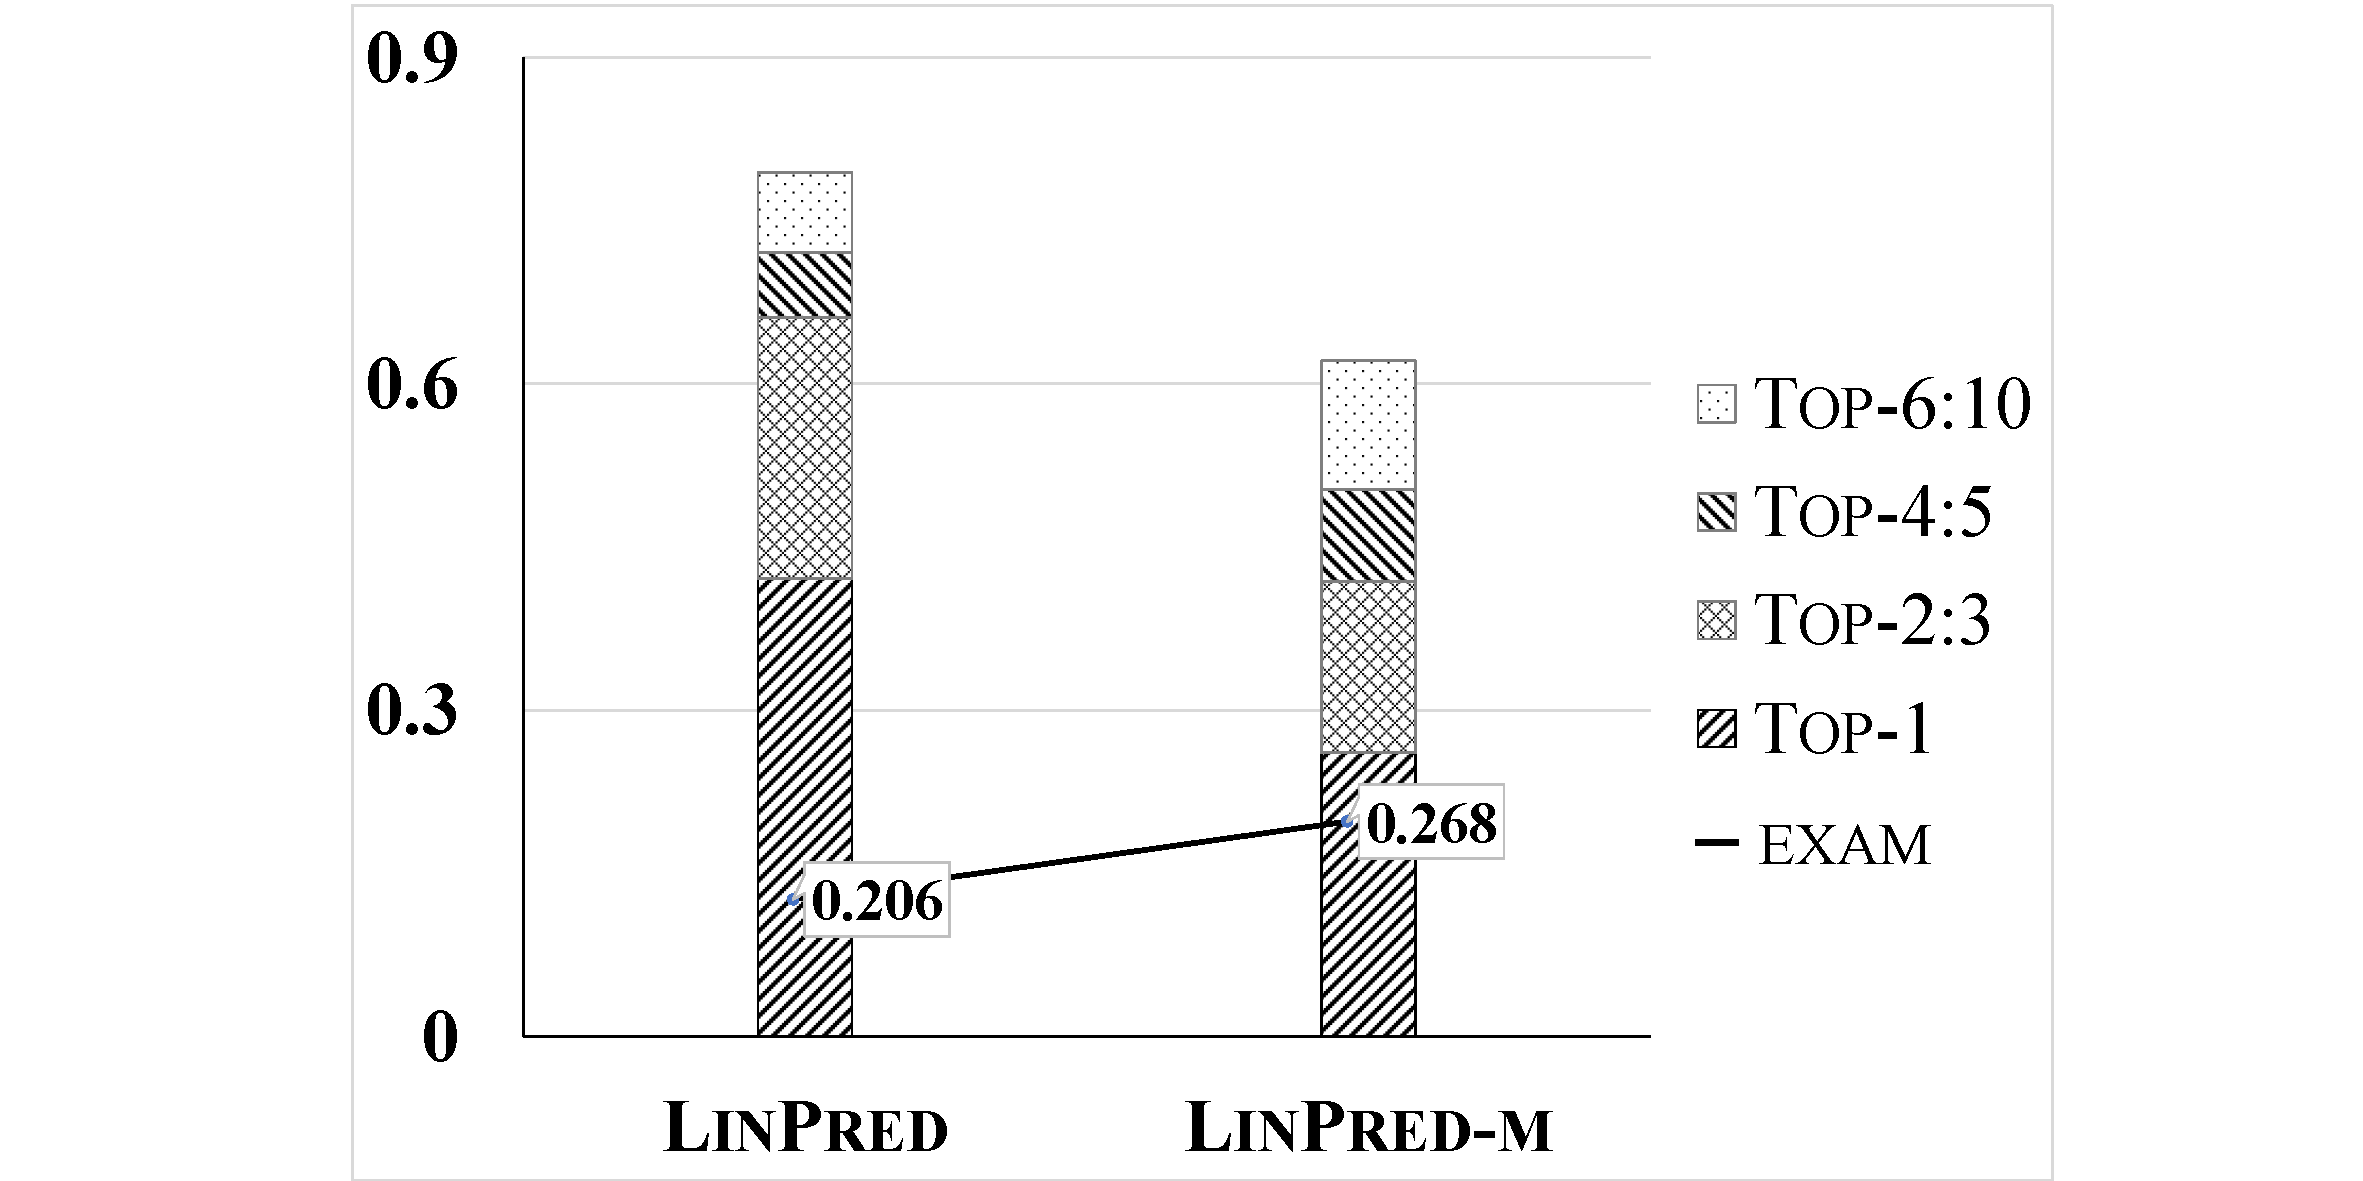
\includegraphics[width=12cm]{figure/ms-level-compare} 
\caption{语句级别和函数级别数据收集的缺陷定位效果对比} 
\label{fig:ms-level-compare}
\end{figure}

数据收集粒度变细之后,谓词数量会增多。
为了进一步探索增加谓词之后缺陷定位的效率是否会受到影响,
本文比较了在语句级别收集数据和在函数级别收集数据的执行时间。
我们发现,平均来说\textsc{LinPred}的谓词数量大约是\textsc{LinPred-m}谓词数量的4.1倍,
但是\textsc{LinPred}的执行时间只是\textsc{LinPred-m}的1.4倍。
同时,\textsc{LinPred}的执行时间也是平均在三分钟以内。
相比于提升数据收集粒度、降低谓词数量,在语句级别收集数据并不会严重地影响性能,同时能带来极大的效果提升。

\subsection{不同的怀疑度计算公式}

本小节将分析比较不同的怀疑度公式对缺陷定位结果的影响,并回答第二个研究问题。
在章\ref{sec:exp_all_formula}中,我们使用了七个怀疑度公式。
然而 SOBER 公式因为插装的内容较多,导致出现“code too large”的编译错误的项目较多,所以将 SOBER 公式排除。
因此剩下五种基于频谱的缺陷定位公式和一种基于状态覆盖的缺陷定位公式。

实验结果如图\ref{fig:formulas}。
图中展示的是每个怀疑度公式的 Top-k 和 EXAM 分数。
图中的“SD”表示的是统计性调试的结果。
从实验结果可以看出,前五个基于频谱的缺陷定位公式并没有太大的差别,
这和之前的研究结果一致。
相比之下Ochiai效果最好。
统计性调试的结果则表现不理想。
可以发现,把基于频谱的缺陷定位公式应用于统计性调试的
预定义谓词后,其效果优于统计性调试的缺陷定位公式效果。

\finding{基于频谱的缺陷定位公式的效果优于基于状态覆盖的缺陷定位公式效果}

\begin{figure}[htbp] 
\centering 
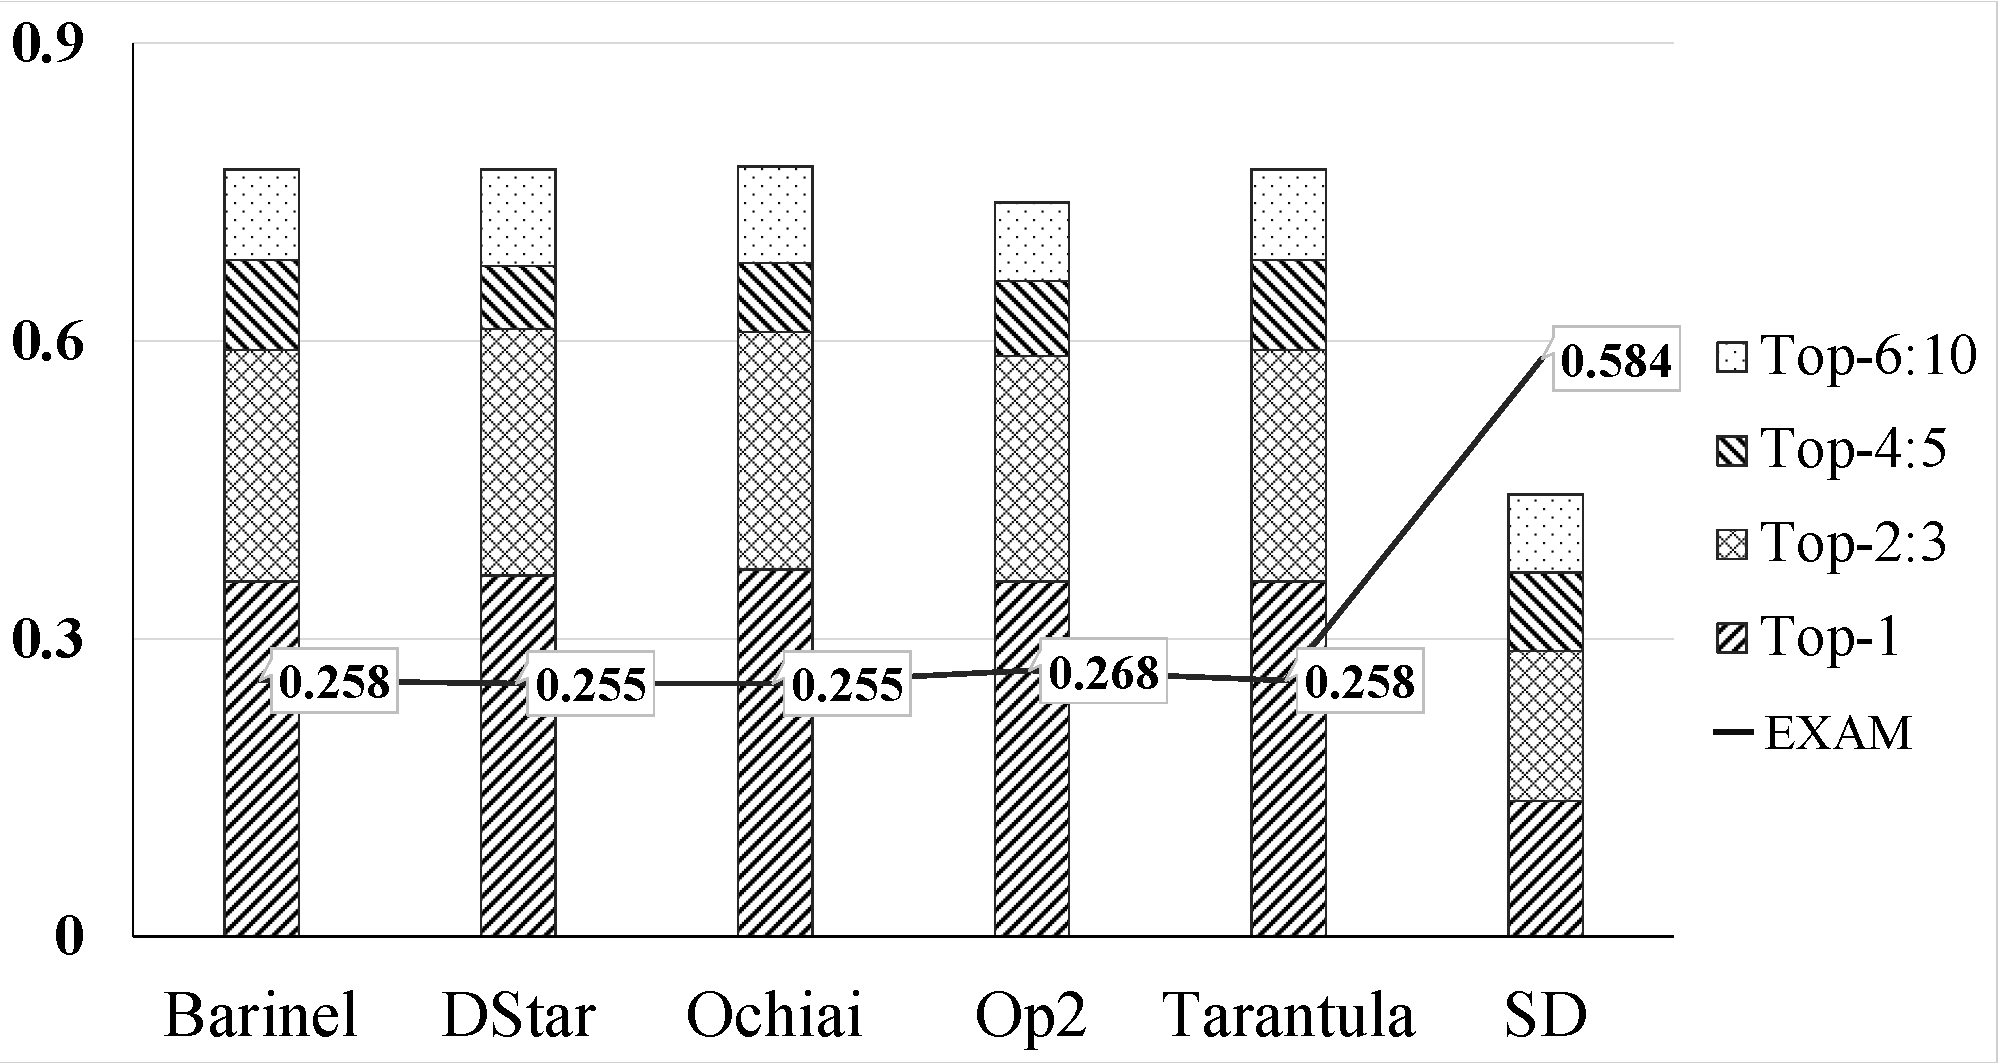
\includegraphics[width=12cm]{figure/formulas} 
\caption{不同怀疑度公式的效果对比} 
\label{fig:formulas}
\end{figure}

为了深入分析基于状态覆盖的缺陷定位公式效果不好的原因,
我们手动分析了统计性调试效果不好的缺陷。
我们发现这是由于很多缺陷都只有一个失败的测试用例,这导致一个谓词的真分支往往只被一个失败的测试用例覆盖。
这会导致统计性调试的公式中$t_f = 1$,导致$log(t_f) = 0$,然后$\frac{log(F)}{log(t_f)} = INF$,
于是最终计算得到的怀疑度为0。
这样谓词本身已经失去了甄别缺陷的能力,仅仅因为测试用例的数量就导致很多谓词的怀疑度为零。
而统计性调试在此前的实验中有效是因为此前的实验对象中一个缺项往往对应多个失败的测试用例。
比如在Liblit\parencite{Liblit2005Scalable}的实验中,对每一个研究对象生成32000个随机输入。
其测试用例数量远远大于 Defects4j 这样的实际项目。
而基于频谱的缺陷定位公式却仍然能够在失败测试用例数量少的情况下得到比较靠谱的结果,
因为它对失败测试用例数量的依赖没有基于状态覆盖的缺陷定位公式的高。
统计性调试公式仍然有它的应用场景。
在使用缺陷定位公式时,可以根据其应用场景选择合适的公式。

\subsection{不同的结合方式}

本小节将深入探讨不同的结合方式,来回答第三个研究问题。
结合的方式被分为了两种\textsc{MaxPred}和\textsc{LinPred}。
图\ref{fig:diff-comb-compare}展示了不同结合方式的 Top-k 和 EXAM 结果。
“SBFL”表示传统的基于频谱的缺陷定位的结果(谓词恒为真),这里的\textsc{MaxPred}的谓词使用预定义谓词。

\begin{figure}[htbp] 
\centering 
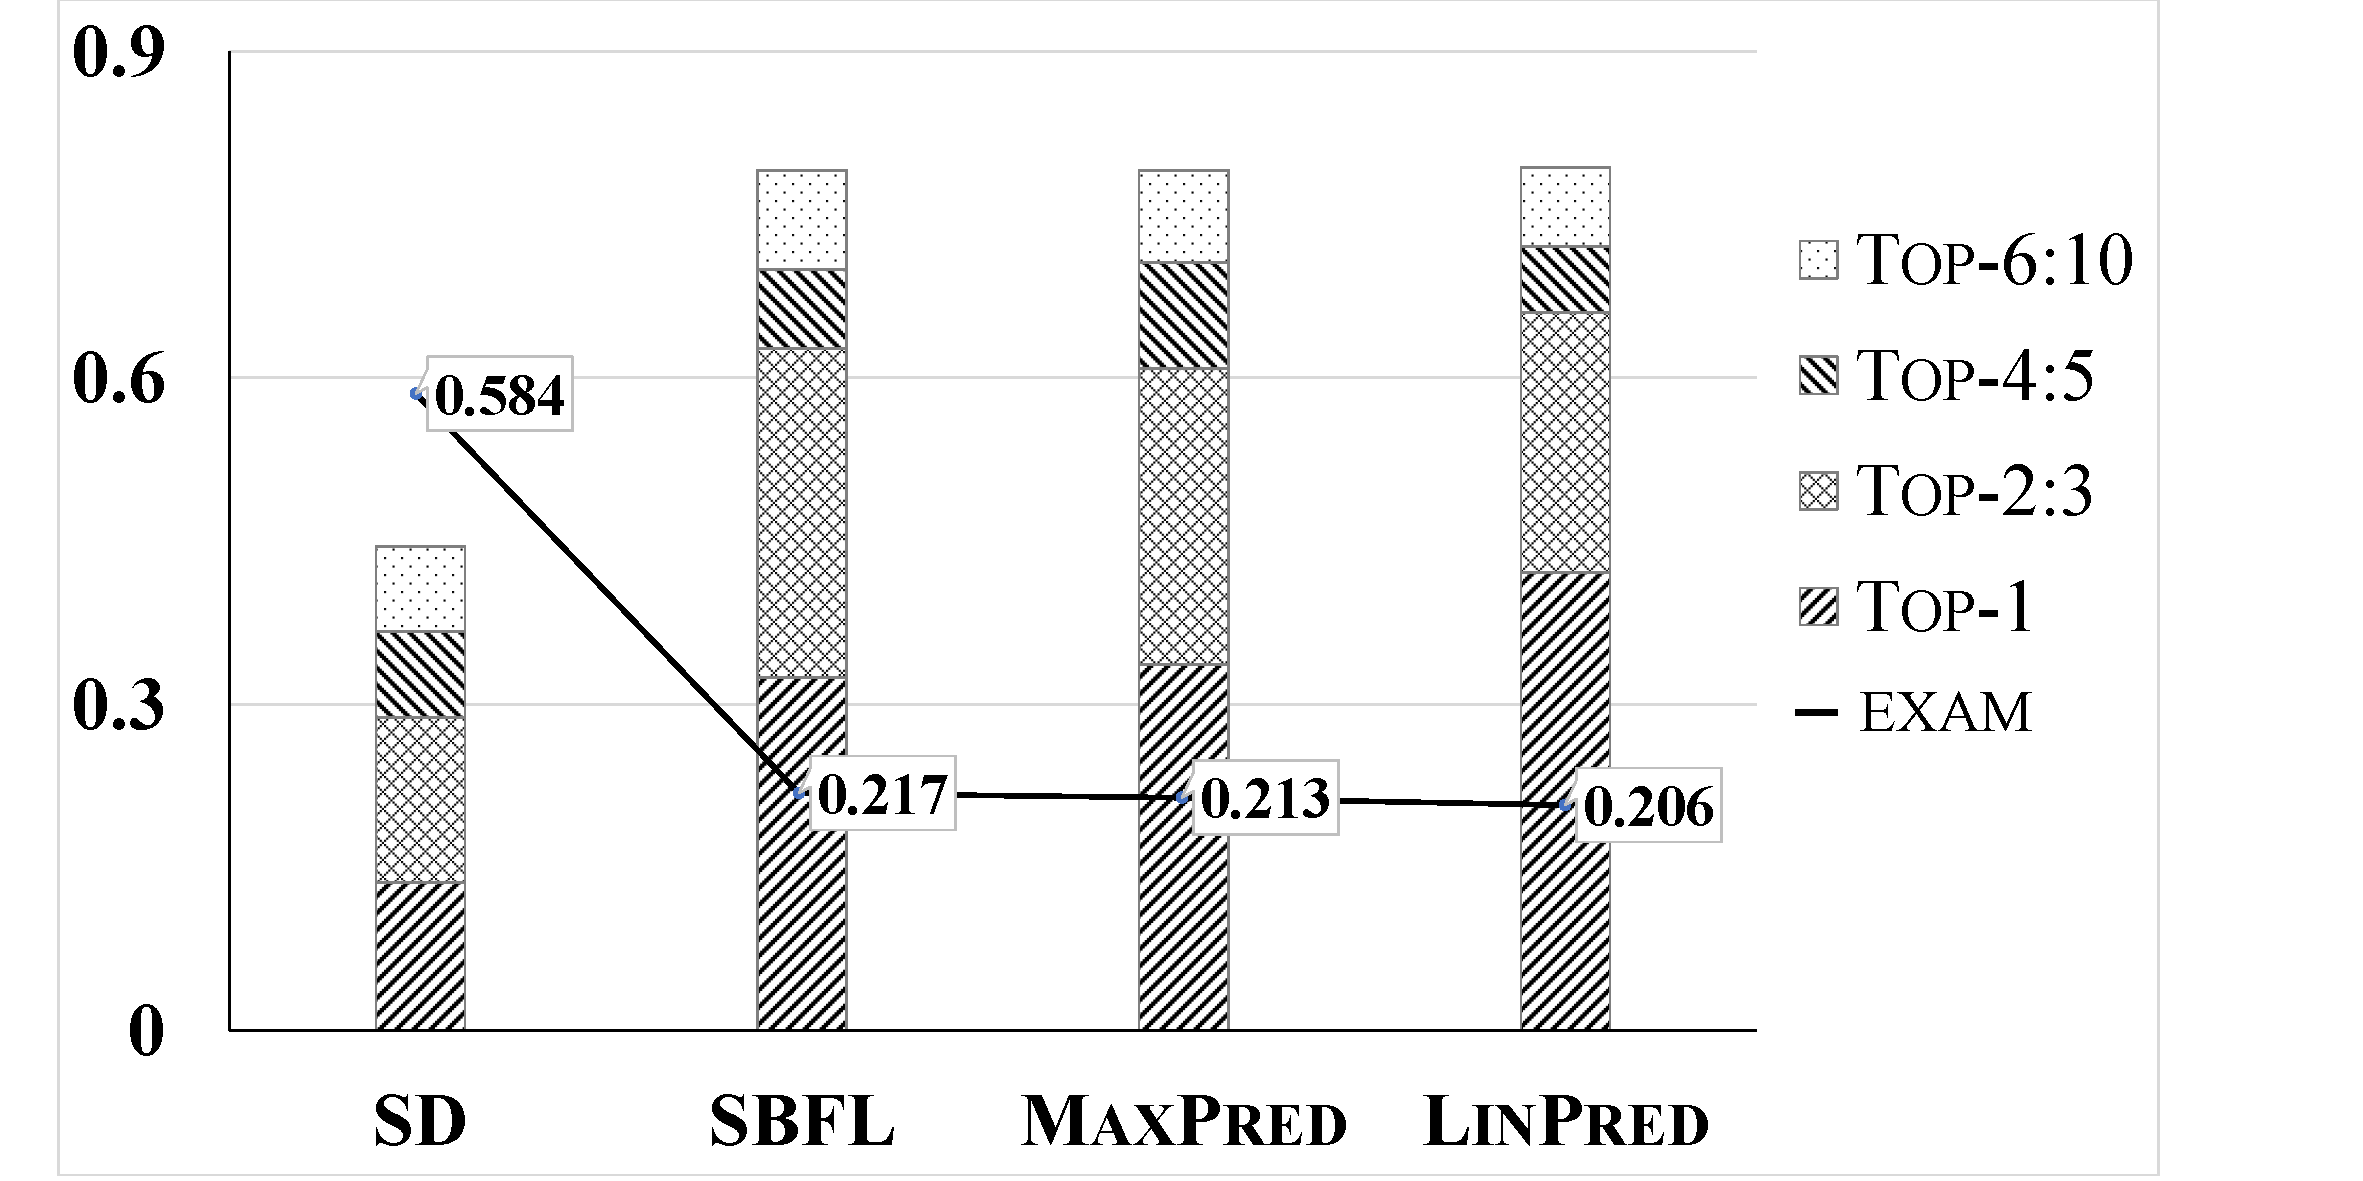
\includegraphics[width=12cm]{figure/diff-comb-compare} 
\caption{不同的结合方式的对比} 
\label{fig:diff-comb-compare}
\end{figure}

从图中可以看出,结合后的\textsc{MaxPred}和\textsc{LinPred}在 Top-1 上优于
原始的方法。
\textsc{LinPred}不仅获得了最好的 Top-k(k=1,3,5,10)值,还拥有最好的 EXAM 值。
\textsc{LinPred}在 Top-1 上与传统的统计性调试比提升了208.9\%,
与基于频谱的缺陷定位比提升了29.9\%。
可见 SBFL 和 \textsc{MaxPred} 结合之后的\textsc{LinPred}效果非常好。

图\ref{fig:diff-comb-compare}中的\textsc{LinPred}采用的默认的$\alpha = 0.5$。
为了分析 SBFL 和 \textsc{MaxPred} 哪一种对结果的影响更大,
采用不同的$\alpha$值进行实现,结果如图\ref{fig:coefficient}。

\begin{figure}[htbp] 
\centering 
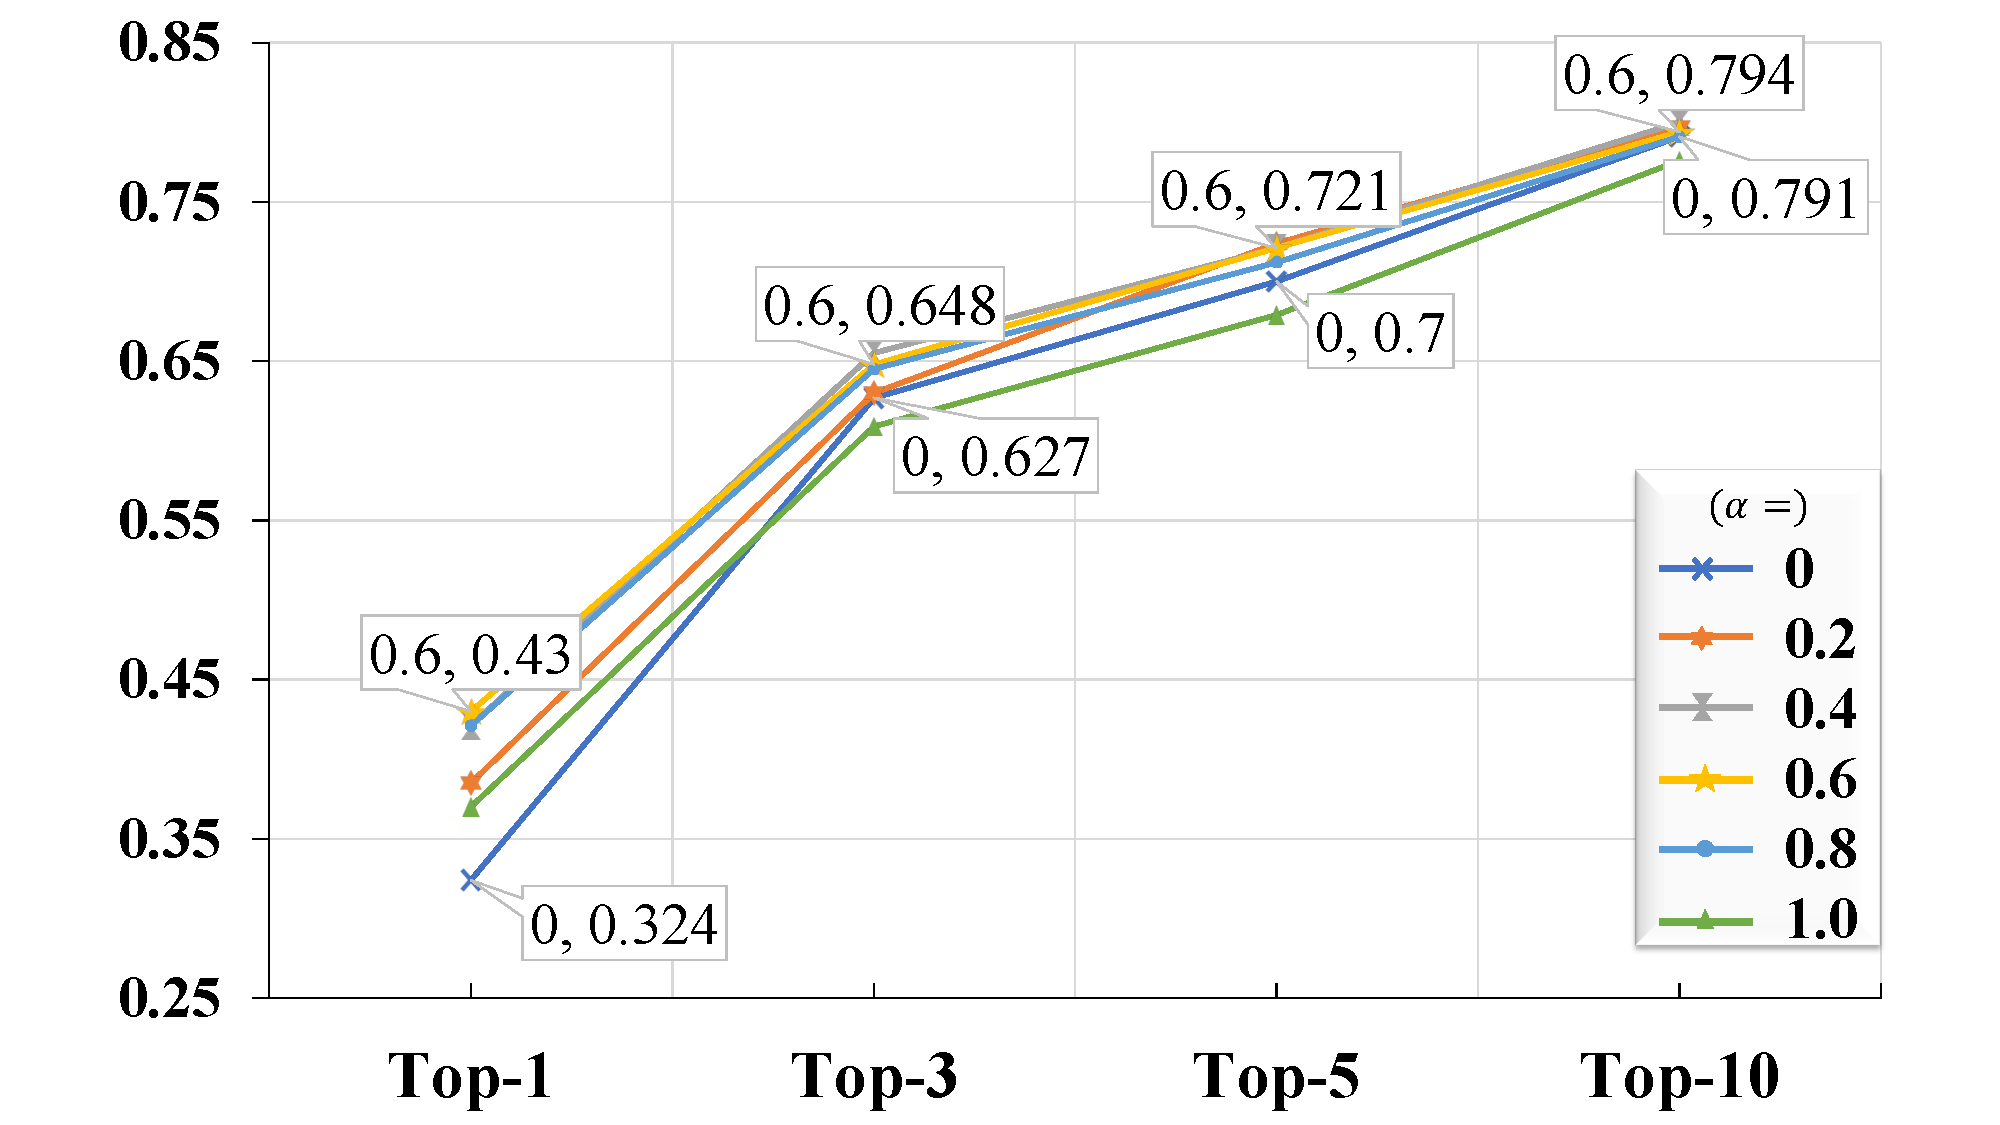
\includegraphics[width=12cm]{figure/coefficient} 
\caption{\textsc{LinPred}中$\alpha$取不同值时,其 Top-k 值的变化情况} 
\label{fig:coefficient}
\end{figure}

从图中可以看出,\textsc{LinPred}总是比原始的 SBFL 方法($\alpha = 0$)在 Top-1 上的效果好。
在 Top-k(k=3,5,10)上,\textsc{MaxPred}的效果一直垫底,
可见\textsc{MaxPred}虽然能给出比较不错的分数,但是单一的\textsc{MaxPred}无法突出缺陷的语句,需要 SBFL 和它互补。
当$\alpha$落在[0.4-0.8]之间的时候,\textsc{LinPred}的效果最好。
不过总体上来说$\alpha$值的影响不会太大。

图\ref{fig:all-figure-method-level}展示了
\textsc{MaxPred},\textsc{LinPred},基于频谱的缺陷定位和基于状态覆盖的缺陷定位
在 Defects4j 上各个项目、各个公式上 Top-1 的结果。
可以看到\textsc{LinPred}在各个项目、各个公式上都有比较好的效果。

\begin{figure}[htbp] 
\centering 
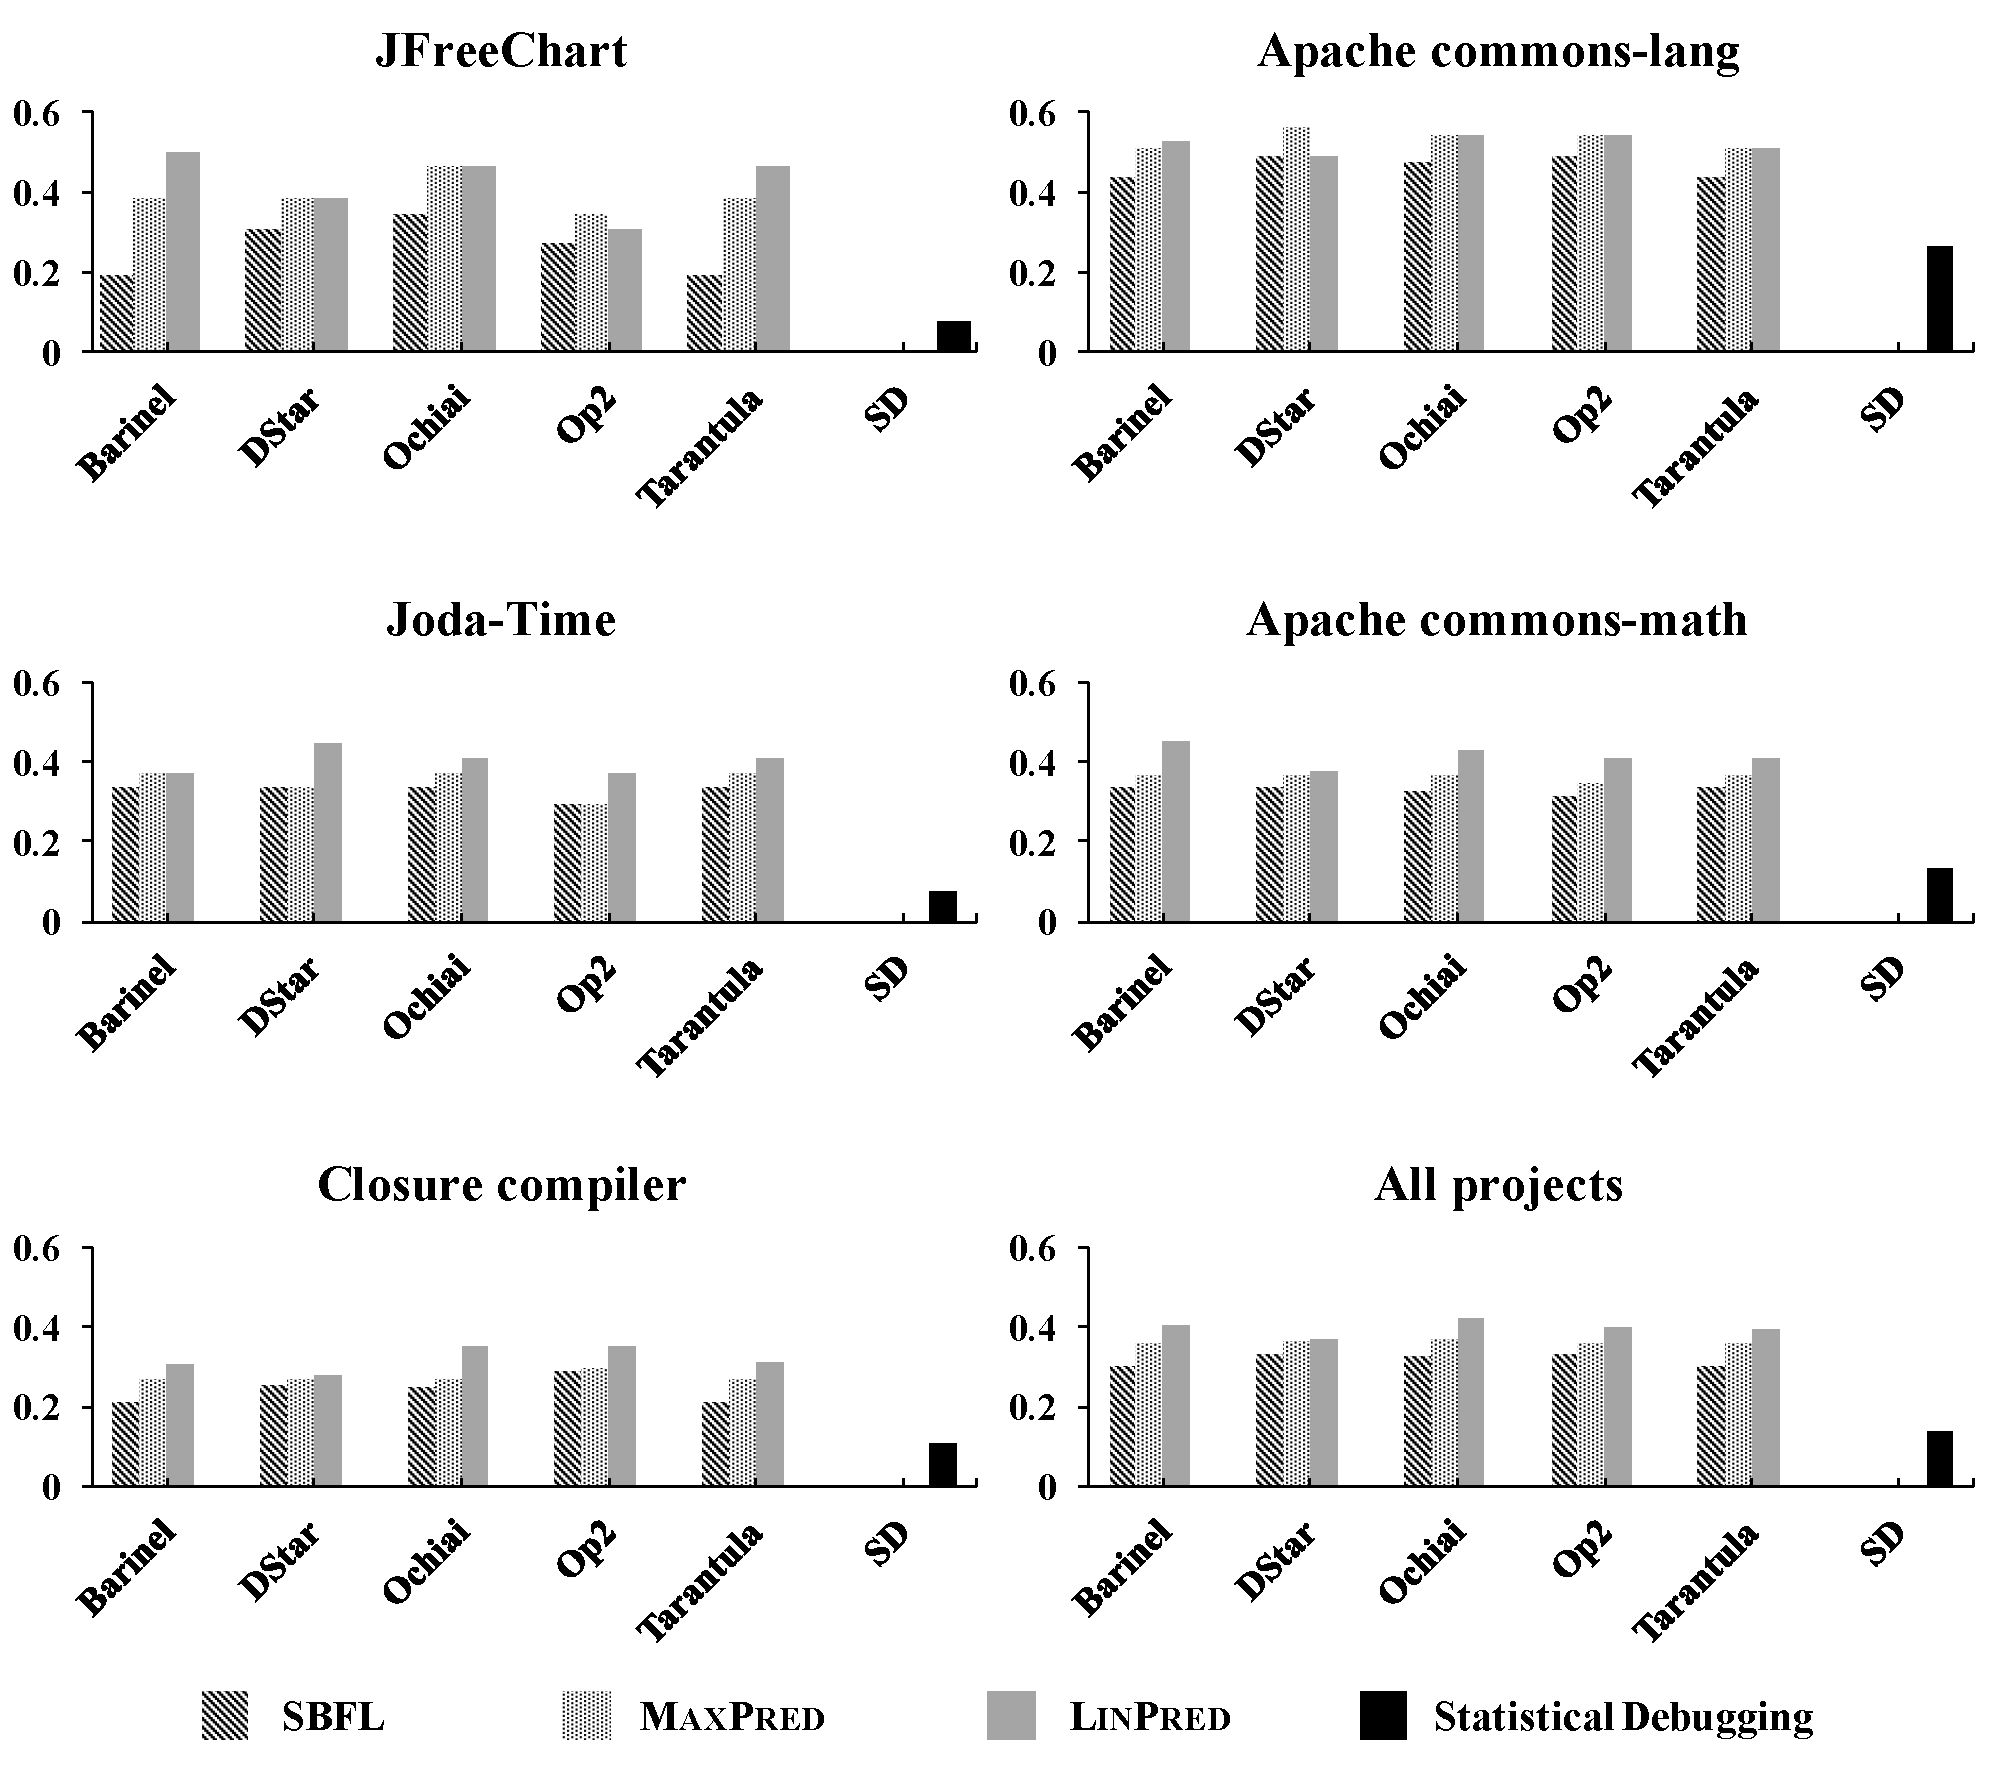
\includegraphics[width=15cm]{figure/all-figure-method-level} 
\caption{\textsc{MaxPred}、\textsc{LinPred}和传统的基于频谱和基于状态覆盖的缺陷定位在各个项目、各个公式上的 Top-1 结果对比} 
\label{fig:all-figure-method-level}
\end{figure}

\subsection{基于机器学习的谓词预测模型效果}

本小节将对基于神经网络的谓词预测模型和基于随机森林的谓词预测模型的预测效果进行研究,
并回答第四个研究问题。

为了考察谓词预测模型的效果,使用验证模型,
即在章\ref{sec:gen_pred_impl}中描述的验证阶段。

先考虑VAR模型。
VAR模型的结果如表\ref{var_predict_result}所示。
整体上来看,随机森林模型的准确率、查准率、查全率和F1分数都比神经网络模型的高。
所有项目的随机森林模型的测试集准确率为86.71\%,
神经网络模型的为82.93\%,略低于随机森林模型。
所有项目的随机森林模型的测试集F1分数为86.39\%,
神经网络模型的为82.20\%。
各个项目神经网络模型的测试集准确率在79.15\%到89.00\%之间波动,
F1分数在78.10\%到88.25\%之间波动。
各个项目随机森林模型的测试集准确率在85.52\%到92.81\%之间波动,
F1分数在83.63\%到92.72\%之间波动。
两个模型的结果比较接近,且效果均较好。

\begin{table}[!tbp]
\centering
\begin{tabular}{|l|l|l|l|l|l|l|l|l|}
\hline
\multirow{2}*{项目} & \multicolumn{4}{c|}{神经网络模型} & \multicolumn{4}{c|}{随机森林模型} \\
\cline{2-9}
& 准确率 & 查准率 & 查全率 & F1分数 & 准确率 & 查准率 & 查全率 & F1分数 \\
\hline
\multirow{2}*{Math} & 85.31\% & 85.46\% & 85.31\% & 84.69\% & 89.10\% & 88.79\% & 89.10\% & 88.84\% \\
\cline{2-9}
& 89.55\% & 90.29\% & 89.55\% & 89.13\% & 97.74\% & 97.73\% & 97.74\% & 97.73\% \\
\hline
\multirow{2}*{Chart} & 89.00\% & 89.05\% & 89.00\% & 88.25\% & 92.81\% & 92.67\% & 92.81\% & 92.72\% \\
\cline{2-9}
& 90.82\% & 91.28\% & 90.82\% & 90.17\% & 97.89\% & 97.89\% & 97.89\% & 97.89\% \\
\hline
\multirow{2}*{Lang} & 83.86\% & 83.85\% & 83.86\% & 83.46\% & 85.52\% & 85.38\% & 85.52\% & 85.37\% \\
\cline{2-9}
& 90.13\% & 90.50\% & 90.13\% & 89.90\% & 96.17\% & 96.16\% & 96.17\% & 96.15\% \\
\hline
\multirow{2}*{Time} & 84.20\% & 84.30\% & 84.20\% & 83.74\% & 86.88\% & 86.80\% & 86.88\% & 86.74\% \\
\cline{2-9}
&  90.34\% & 90.84\% & 90.34\% & 90.04\% & 97.92\% & 97.92\% & 97.92\% & 97.91\% \\
\hline
\multirow{2}*{Closure} & 79.15\% & 79.12\% & 79.15\% & 78.10\% & 84.15\% & 83.52\% & 84.15\% & 83.63\% \\
\cline{2-9}
& 85.23\% & 86.31\% & 85.23\% & 84.57\% & 96.71\% & 96.69\% & 96.71\% & 96.68\% \\
\hline
\multirow{2}*{全部} & 82.93\% & 82.98\% & 82.93\% & 82.20\% & 86.71\% & 86.34\% & 86.71\% & 86.39\% \\
\cline{2-9}
& 88.20\% & 88.96\% & 88.20\% & 87.72\% & 97.09\% & 97.08\% & 97.09\% & 97.08\% \\
\hline
\end{tabular}
\caption{VAR模型的预测效果,每个项目第一行为测试集结果,第二行为训练集结果}
\label{var_predict_result}
\end{table}

\begin{table}[!tbp]
\centering
\begin{tabular}{|l|l|l|l|l|l|l|l|l|}
\hline
\multirow{2}*{项目} & \multicolumn{4}{c|}{神经网络模型} & \multicolumn{4}{c|}{随机森林模型} \\
\cline{2-9}
& 准确率 & 查准率 & 查全率 & F1分数 & 准确率 & 查准率 & 查全率 & F1分数 \\
\hline
\multirow{2}*{Math} & 26.01\% & 20.69\% & 26.01\% & 21.13\% & 50.51\% & 48.44\% & 50.51\% & 47.57\% \\
\cline{2-9}
& 34.19\% & 27.02\% & 34.19\% & 27.59\% & 84.07\% & 83.60\% & 84.07\% & 82.27\% \\
\hline
\multirow{2}*{Chart} & 39.42\% & 37.33\% & 39.42\% & 37.02\% & 49.44\% & 47.14\% & 49.44\% & 47.29\%\\
\cline{2-9}
& 47.48\% & 44.06\% & 47.48\% & 43.79\% & 83.49\% & 82.82\% & 83.49\% & 82.13\% \\
\hline
\multirow{2}*{Lang} & 42.67\% & 33.42\% & 42.67\% & 36.10\% & 58.93\% & 55.34\% & 58.93\% & 55.80\% \\
\cline{2-9}
& 49.92\% & 38.35\% & 49.92\% & 41.63\% & 85.76\% & 83.96\% & 85.76\% & 83.80\%\\
\hline
\multirow{2}*{Time} & 43.74\% & 33.31\% & 43.74\% & 36.87\% & 65.82\% & 62.10\% & 65.82\% & 62.63\%\\
\cline{2-9}
& 48.72\% & 36.08\% & 48.72\% & 40.14\% & 93.61\% & 92.92\% & 93.61\% & 92.66\%\\
\hline
\multirow{2}*{Closure} & 24.76\% & 19.47\% & 24.76\% & 20.98\% & 36.58\% & 32.20\% & 36.58\% & 32.98\%\\
\cline{2-9}
& 33.04\% & 25.43\% & 33.04\% & 27.40\% & 85.77\% & 85.34\% & 85.77\% & 84.35\% \\
\hline
\multirow{2}*{全部} & 30.90\% & 24.72\% & 30.90\% & 26.15\% & 47.93\% & 44.58\% & 47.93\% & 44.75\% \\
\cline{2-9}
& 38.69\% & 30.41\% & 38.69\% & 32.20\% & 85.69\% & 84.96\% & 85.69\% & 84.10\% \\
\hline
\end{tabular}
\caption{EXPR模型的预测效果,每个项目第一行为测试集结果,第二行为训练集结果}
\label{expr_predict_result}
\end{table}

再分析EXPR模型。
EXPR模型的预测结果如表\ref{expr_predict_result}。
随机森林模型仍然比神经网络效果更好,且差距相比VAR模型更大。
神经网络模型的所有项目的训练集准确率都仅为38.69\%,
虽然是一个多分类问题,但是数值仍然偏低。
测试集准确率只有30.90\%。
随机森林模型的所有项目的训练集准确率虽然有 85.69\% ,
但是测试集的准确率只有 47.93\%。
EXPR模型还有很大的提升空间。
随机森林的效果比神经网络的效果好,可能是因为
数据量不够很好地支撑神经网络的运算。
神经网络的学习需要大量的数据,
而随机森林可以从较少的数据中学习。
随机森林的测试集准确率不如训练集准确率,
可能是由于谓词分布不均衡导致,
因为随机森林本身是一个控制了过拟合的模型。

然后考虑预测模型的执行时间。
这里计算的是章\ref{sec:gen_pred_impl}中验证阶段的时间,
其时间和训练阶段时间基本一致。
随机森林模型的平均训练时间为23秒,
而神经网络模型的平均训练时间为1382秒,
约为23分钟。
可见神经网络的训练时间远远高于随机森林模型的训练时间,几乎为其60倍,
而且其准确率等指标效果不如随机森林模型。

\subsection{不同谓词对结果的影响}

在之前的研究问题的分析中,我们已经发现了使用预定义谓词的\textsc{LinPred}具有非常好的效果。
相比于基于频谱的缺陷定位,\textsc{LinPred}利用了谓词进行进一步的状态划分。
在本小节,我们将会深入探究谓词在缺陷定位中起的作用,并且考虑上基于机器学习方法预测出来的谓词,来回答第五个研究问题。

谓词在项目中的平均数量如表\ref{pred_number}所示。 
Closure 因为项目较大所以谓词数量较多。
各个谓词类型上来看,
预定义谓词数量最多,其次是恒真谓词和预测谓词(随机森林),预测谓词(神经网络)谓词数量最少。
预定义谓词的数量大约是预测谓词(神经网络)的5.6倍。
虽然预定义谓词数量多,但是因为预定义谓词的收集时间非常快(AST遍历时间),
与平均训练时间约为23分钟的神经网络模型相比,效率仍然很高。

\begin{table}
\centering
\begin{tabular}{|c|c|c|c|c|c|c|}
\hline
\multirow{2}*{谓词类型} & \multicolumn{6}{c|}{项目} \\
\cline{2-7}
~ & Chart & Lang & Time & Math & Closure & 总计 \\
\hline
预定义谓词 & 913.6 & 119.5 & 1064.2 & 1973.0 & 2426.8 & 1662.8 \\
\hline
预测谓词(随机森林) & 461.3 & 93.8 & 438.8 & 375.8 & 812.1 & 498.0 \\
\hline
预测谓词(神经网络)& 218.5 & 69.6 & 335.9 & 179.2 & 507.9 & 296.4 \\
\hline
恒真谓词 & 566.5 & 75.8 & 892.7 & 278.3 & 3401.3 & 1470.9 \\
\hline
\end{tabular}
\caption{平均每个项目的谓词数量}
\label{pred_number}
\end{table}

\begin{figure}[htbp] 
\centering 
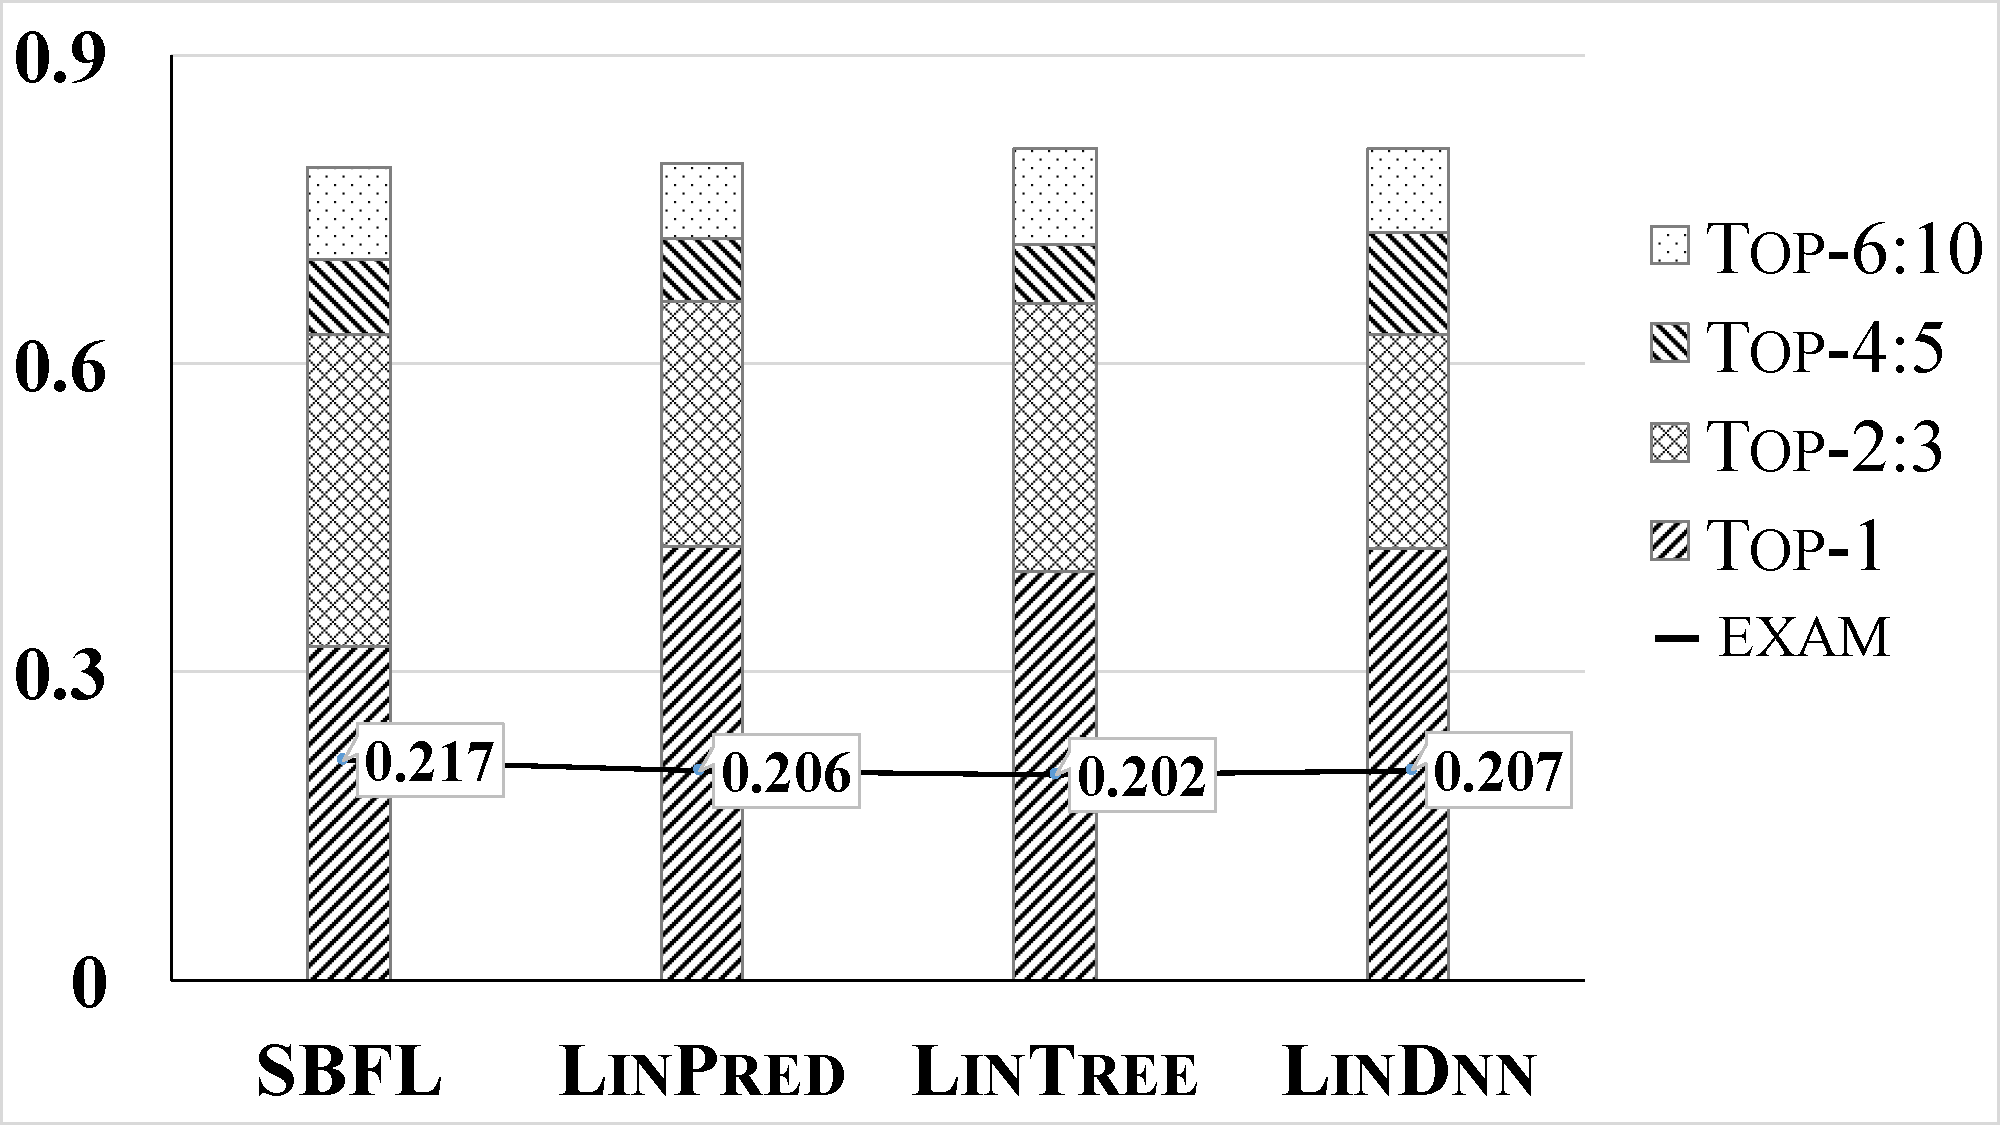
\includegraphics[width=10cm]{figure/diff-ml-pred-compare} 
\caption{预测谓词和预定义谓词的缺陷定位效果对比} 
\label{fig:diff-ml-pred-compare}
\end{figure}

为区分使用不同谓词的\textsc{LinPred},在本研究问题中,把使用预定义谓词的 \textsc{LinPred} 称为\textsc{LinSD}。
\textsc{LinTree}表示使用随机森林模型预测的谓词,
\textsc{LinDnn}表示使用神经网络模型预测的谓词。

首先考虑谓词的实际定位效果。
把使用随机森林模型和神经网络模型预测出的谓词的缺陷定位方法,与使用预定义谓词和恒真谓词的比较,
得到图\ref{fig:diff-ml-pred-compare},Top-k具体数值见表\ref{diff-ml-pred-compare-data}。
从Top-1和Top-3指标上看,\textsc{LinSD}的效果最好。
可见预定义的谓词在把缺陷定位在最前面具有很大优势。
而从EXAM指标上看,\textsc{LinTree}的效果最好。
虽然随机森林模型预测出的谓词在把缺陷排在最前面的效果不如预定义谓词,
但是在整体上随机森林模型预测出的谓词能够把缺陷排在更加靠前的位置。
\textsc{LinTree}模型具有高准确率、高F1值,其结果也具有最低的EXAM值。
说明了基于机器学习的谓词预测在实际中是具有可行性的。
\textsc{LinDnn}在Top-1上效果和\textsc{LinSD}相近,
仅相差一个缺陷。
虽然\textsc{LinDnn}在EXAM指标上不如\textsc{LinTree},
但是Top-1指标上效果比\textsc{LinTree}更好。

\begin{table}
\centering
\begin{tabular}{|l|r|r|r|r|}
\hline
缺陷定位方法 & Top-1 & Top-3 & Top-5 & Top-10 \\
\hline
\textsc{LinSD} & 139 & 218 & 238 & 262 \\
\hline
\textsc{LinTree} & 131 & 217 & 236 & 267 \\
\hline
\textsc{LinDnn} & 138 & 207 & 240 & 267 \\
\hline
\end{tabular}
\caption{预测谓词和预定义谓词的缺陷定位效果对比-具体数值}
\label{diff-ml-pred-compare-data}
\end{table}

\begin{figure}[tbp] 
\centering 
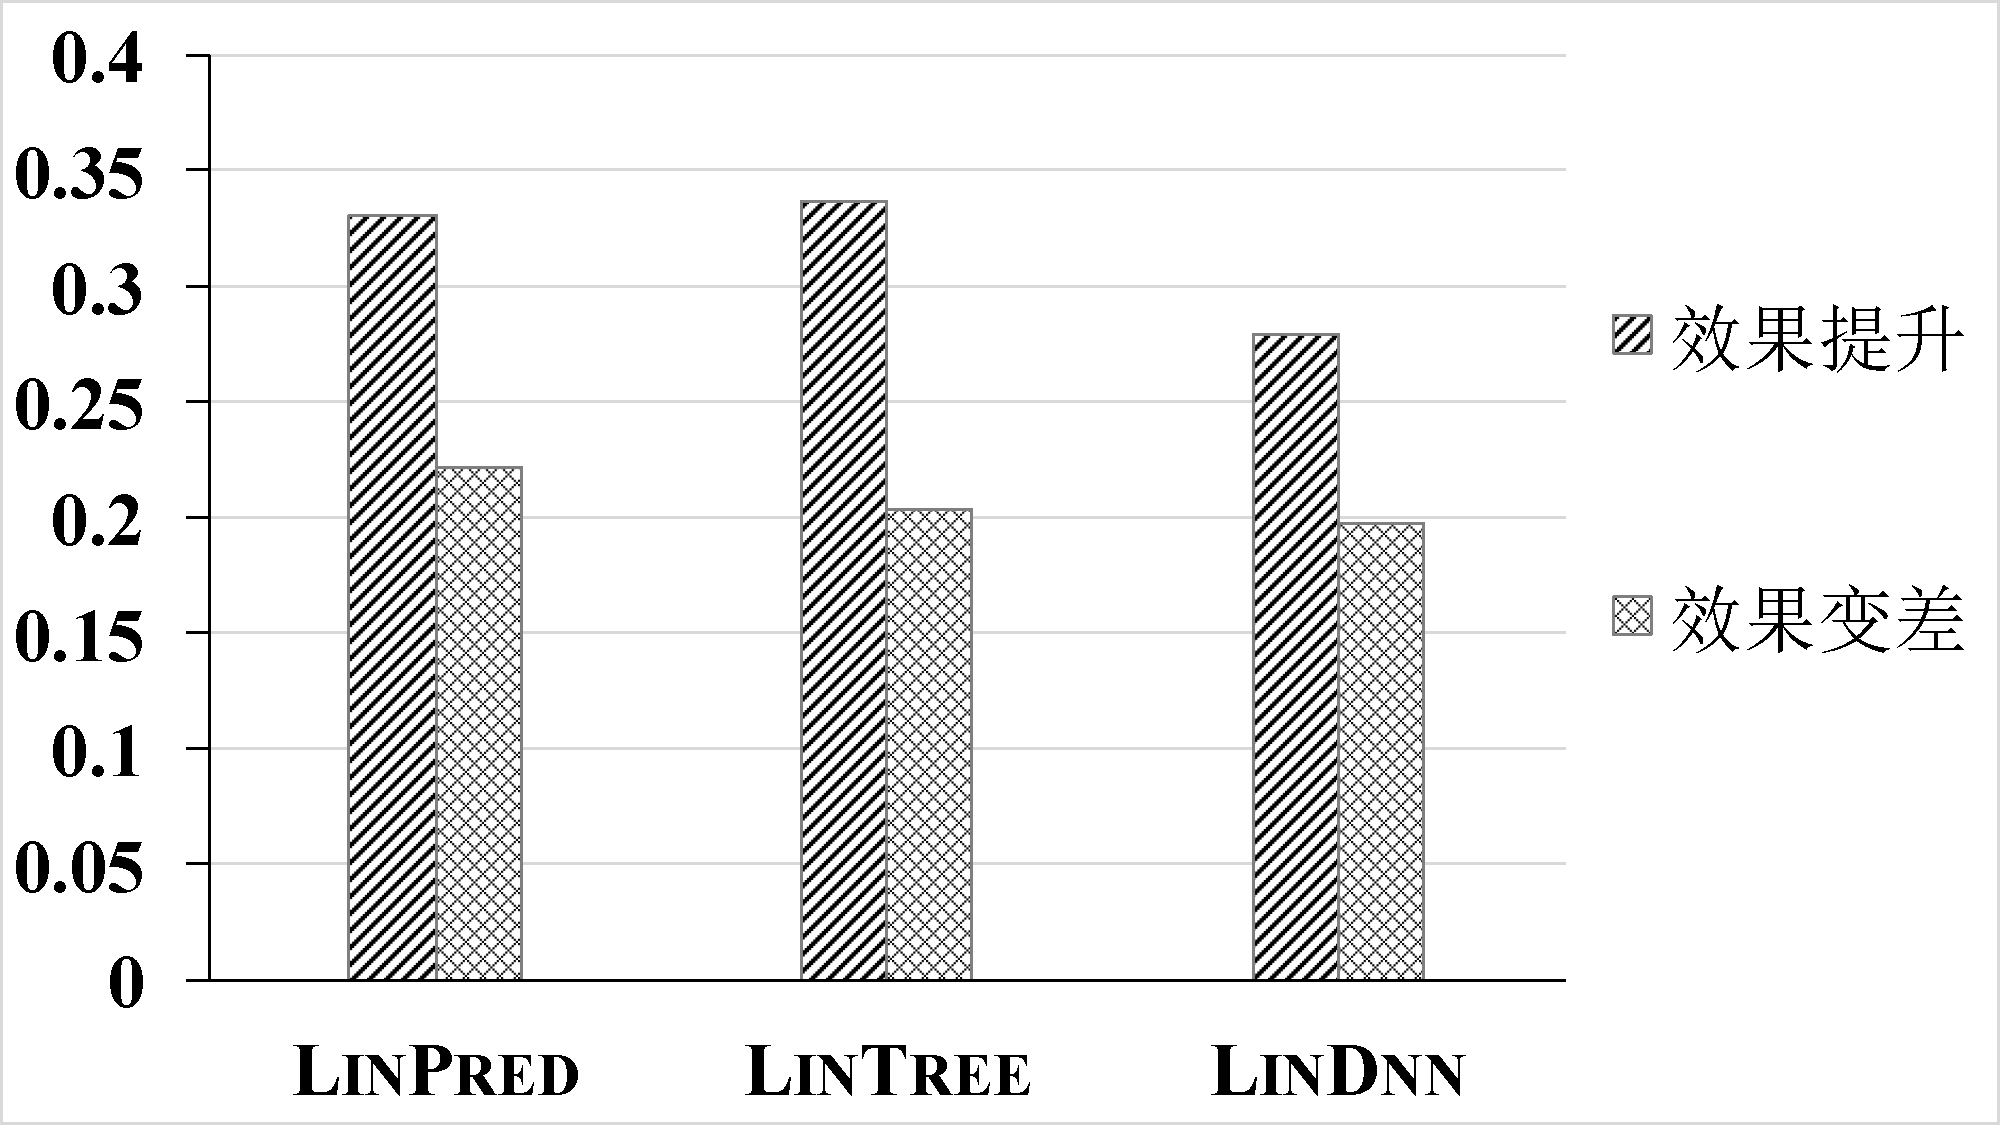
\includegraphics[width=11cm]{figure/improve-deteriorate-all} 
\caption{使用谓词后的缺陷定位效果与原始的基于频谱的缺陷定位相比的提升与下降} 
\label{fig:improve-deteriorate-all}
\end{figure}

然后分析谓词对预测效果是提升还是破坏。
谓词对一个缺陷的定位效果有提升,表示使用这种谓词后,缺陷在怀疑度列表上的位置相比于基于频谱的缺陷定位靠前了。
相反,如果使用这种谓词后,缺陷在怀疑度列表上的位置相比于基于频谱的缺陷定位靠后了,则表示
这种谓词让缺陷定位的效果变差了。
图\ref{fig:improve-deteriorate-all}的纵坐标表示所占总的缺陷的比例,
横坐标表示不同的谓词类型。
左侧为谓词有提升作用的缺陷的比例。
右侧为谓词有破坏作用的缺陷的比例。
使用默认的Ochiai公式。
随机森林在效果提升上最为明显,
其次是预定义谓词,
最后是神经网络预测出的谓词。
但是神经网络预测的谓词让效果变差了的最少。
在实际实验中,
谓词不仅能让效果变好,
也会有具有误导作用的谓词。
说明并不是一味地增加谓词就能取得好的结果,
减少具有误导作用的谓词也很关键。

% 对于程序元素$e$,
% 一个谓词被认为是对定位效果有积极的影响,如果$c_0 > c_1$且$e$是缺陷程序元素,或者$c_0 < c_1$且$e$不是缺陷程序元素。
% 其中$c_0$表示使用预定义谓词的\textsc{MaxPred}的结果,
% $c_1$表示基于频谱的缺陷定位的结果(谓词恒真的\textsc{MaxPred}的结果)。
% 一个谓词被认为是对定位效果有消极影响,如果$c_0 < c_1$且$e$是缺陷程序元素,或者$c_0 > c_1$且$e$不是缺陷程序元素。
% 于是谓词被分为两类(不满足以上两类的属于既没有积极影响,也没有消极影响的谓词),
% 这两类在不同的怀疑度计算公式下的分布情况如图\ref{fig:improve-deteriorate}。
% 可以发现大部分谓词还是对结果有积极影响的,只有少部分会对结果产生不好的影响。

\subsubsection{预定义谓词}

\begin{figure}[htbp] 
\centering 
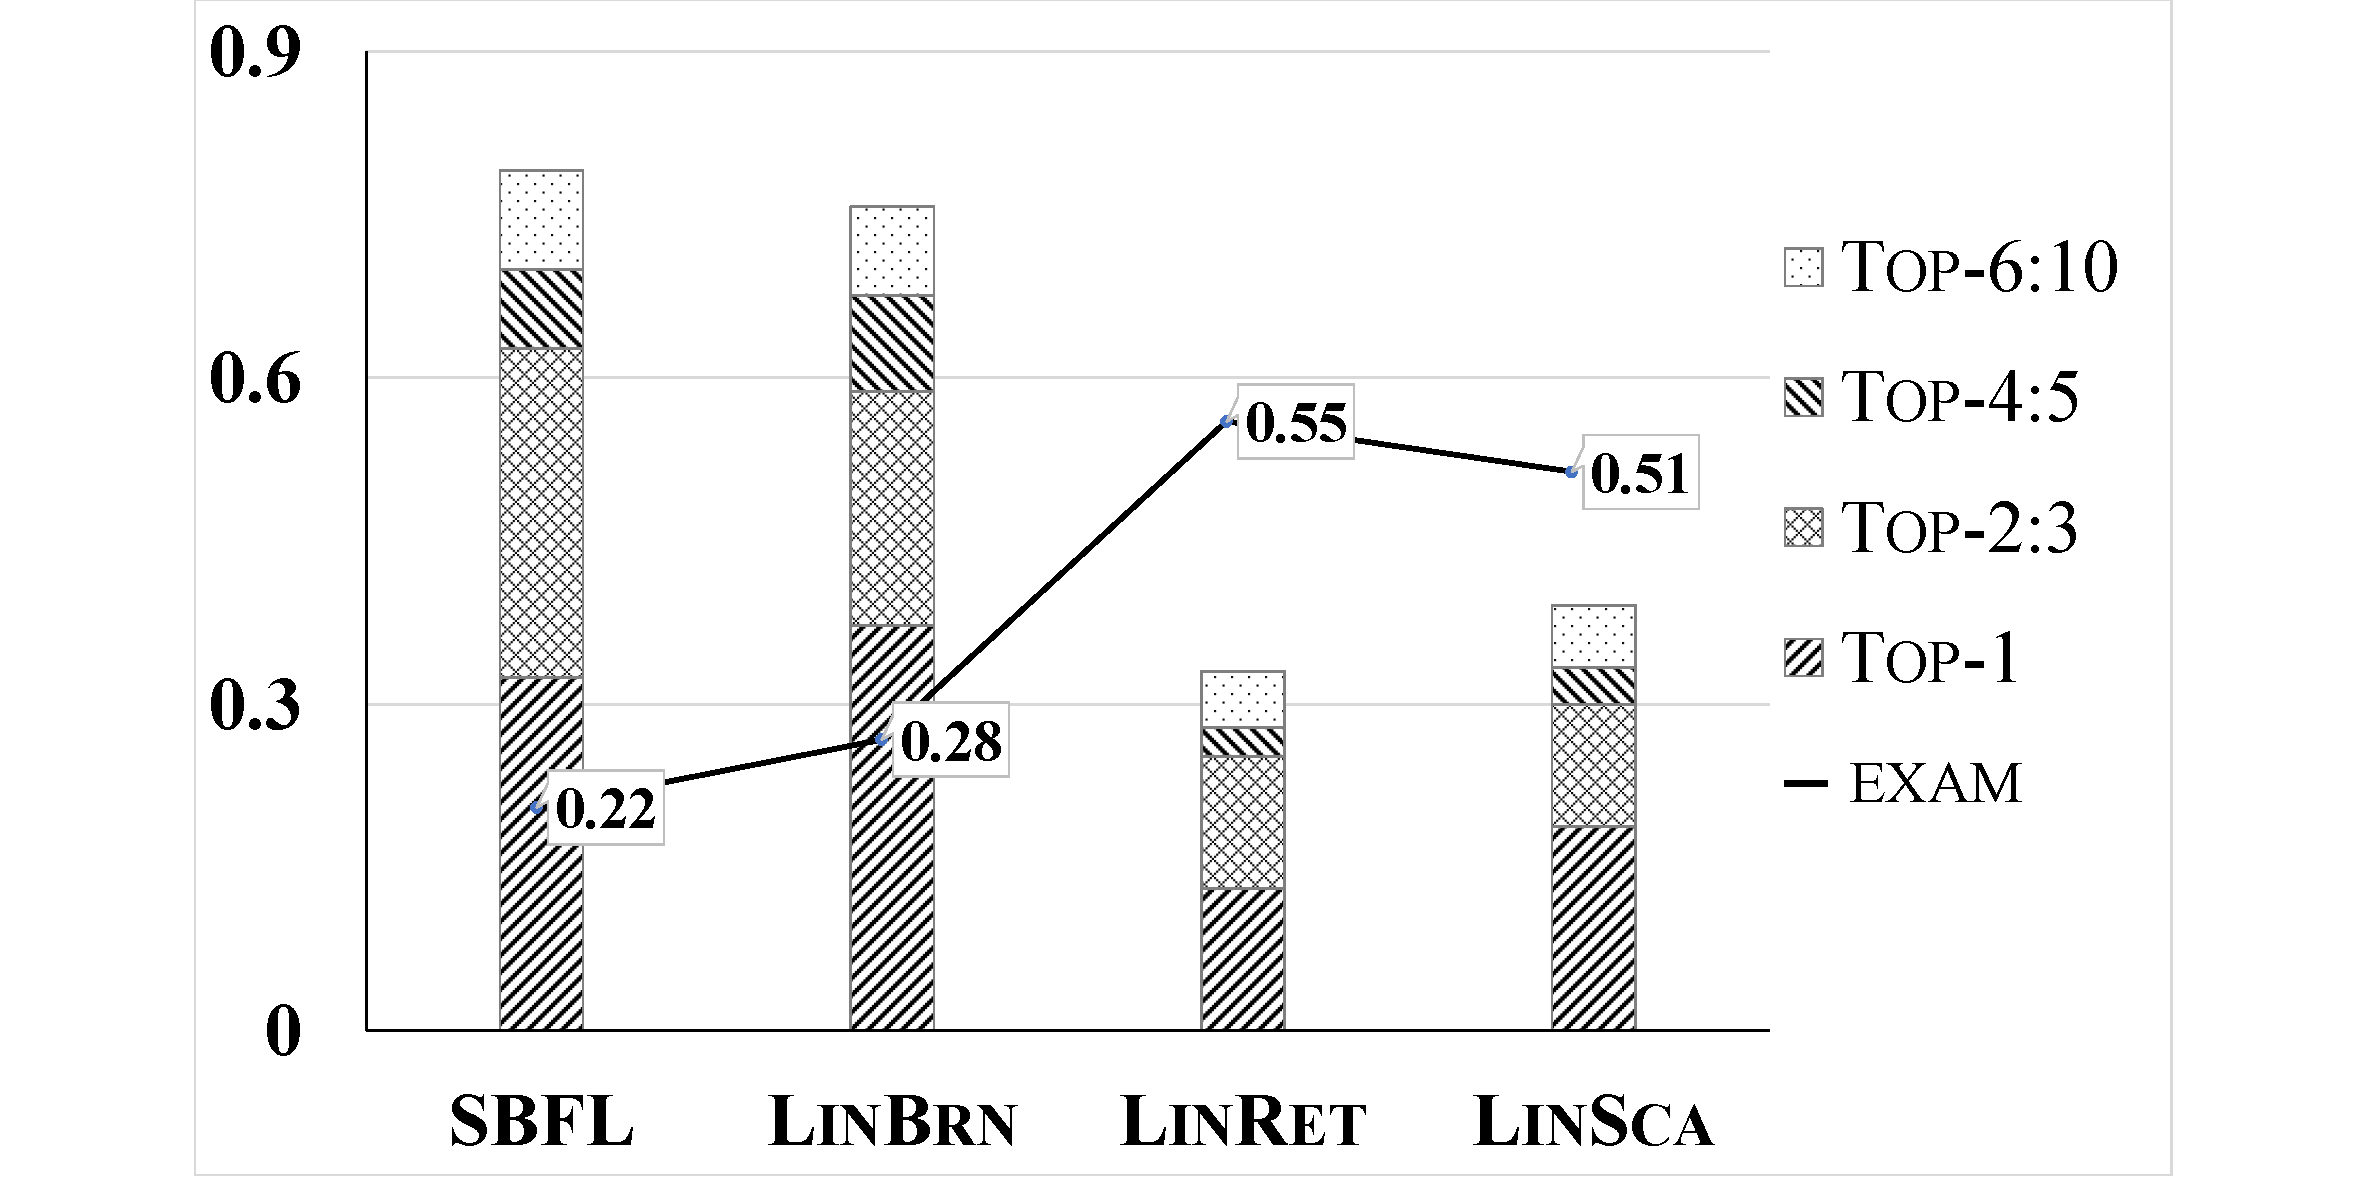
\includegraphics[width=12cm]{figure/diff-predictor-compare} 
\caption{使用不同的预定义谓词的缺陷定位效果对比} 
\label{fig:diff-predictor-compare}
\end{figure}

为了探索是三种预定义谓词中的哪种谓词起了关键作用,
我们把三种预定义谓词分别作为谓词集合,进行实验。
实验结果如图\ref{fig:diff-predictor-compare}所示。
\textsc{LinBrn}表示只使用分支谓词,
\textsc{LinRet}表示只使用返回值谓词,
\textsc{LinSca}表示只使用数值对谓词。
可以发现,\textsc{LinBrn}拥有比\textsc{LinRet}和\textsc{LinSca}更好的 Top-k(k=1,3,5,10)和 EXAM 值。
所以分支谓词的效果最明显。
\textsc{LinBrn}在 Top-1 上的效果比基于频谱的缺陷定位效果还要好,
不过基于频谱的缺陷定位在其他 Top-k 上效果更好,说明了二者的互补性。

\finding{在预定义谓词中,分支谓词对\textsc{LinPred}效果提升最明显。}

为了进一步验证我们的发现,我们比较了使用三种预定义谓词的\textsc{MaxPred}和
只使用了分支谓词的\textsc{MaxPred}(称为\textsc{MaxBranch}),
结果如图\ref{fig:branch-compare}。
可以发现\textsc{MaxPred}和~\textsc{MaxBranch}~的结果非常相近,
虽然\textsc{MaxBranch}少了两种谓词,但是核心的分支谓词起了很大的作用。

\begin{figure}[htbp] 
\centering 
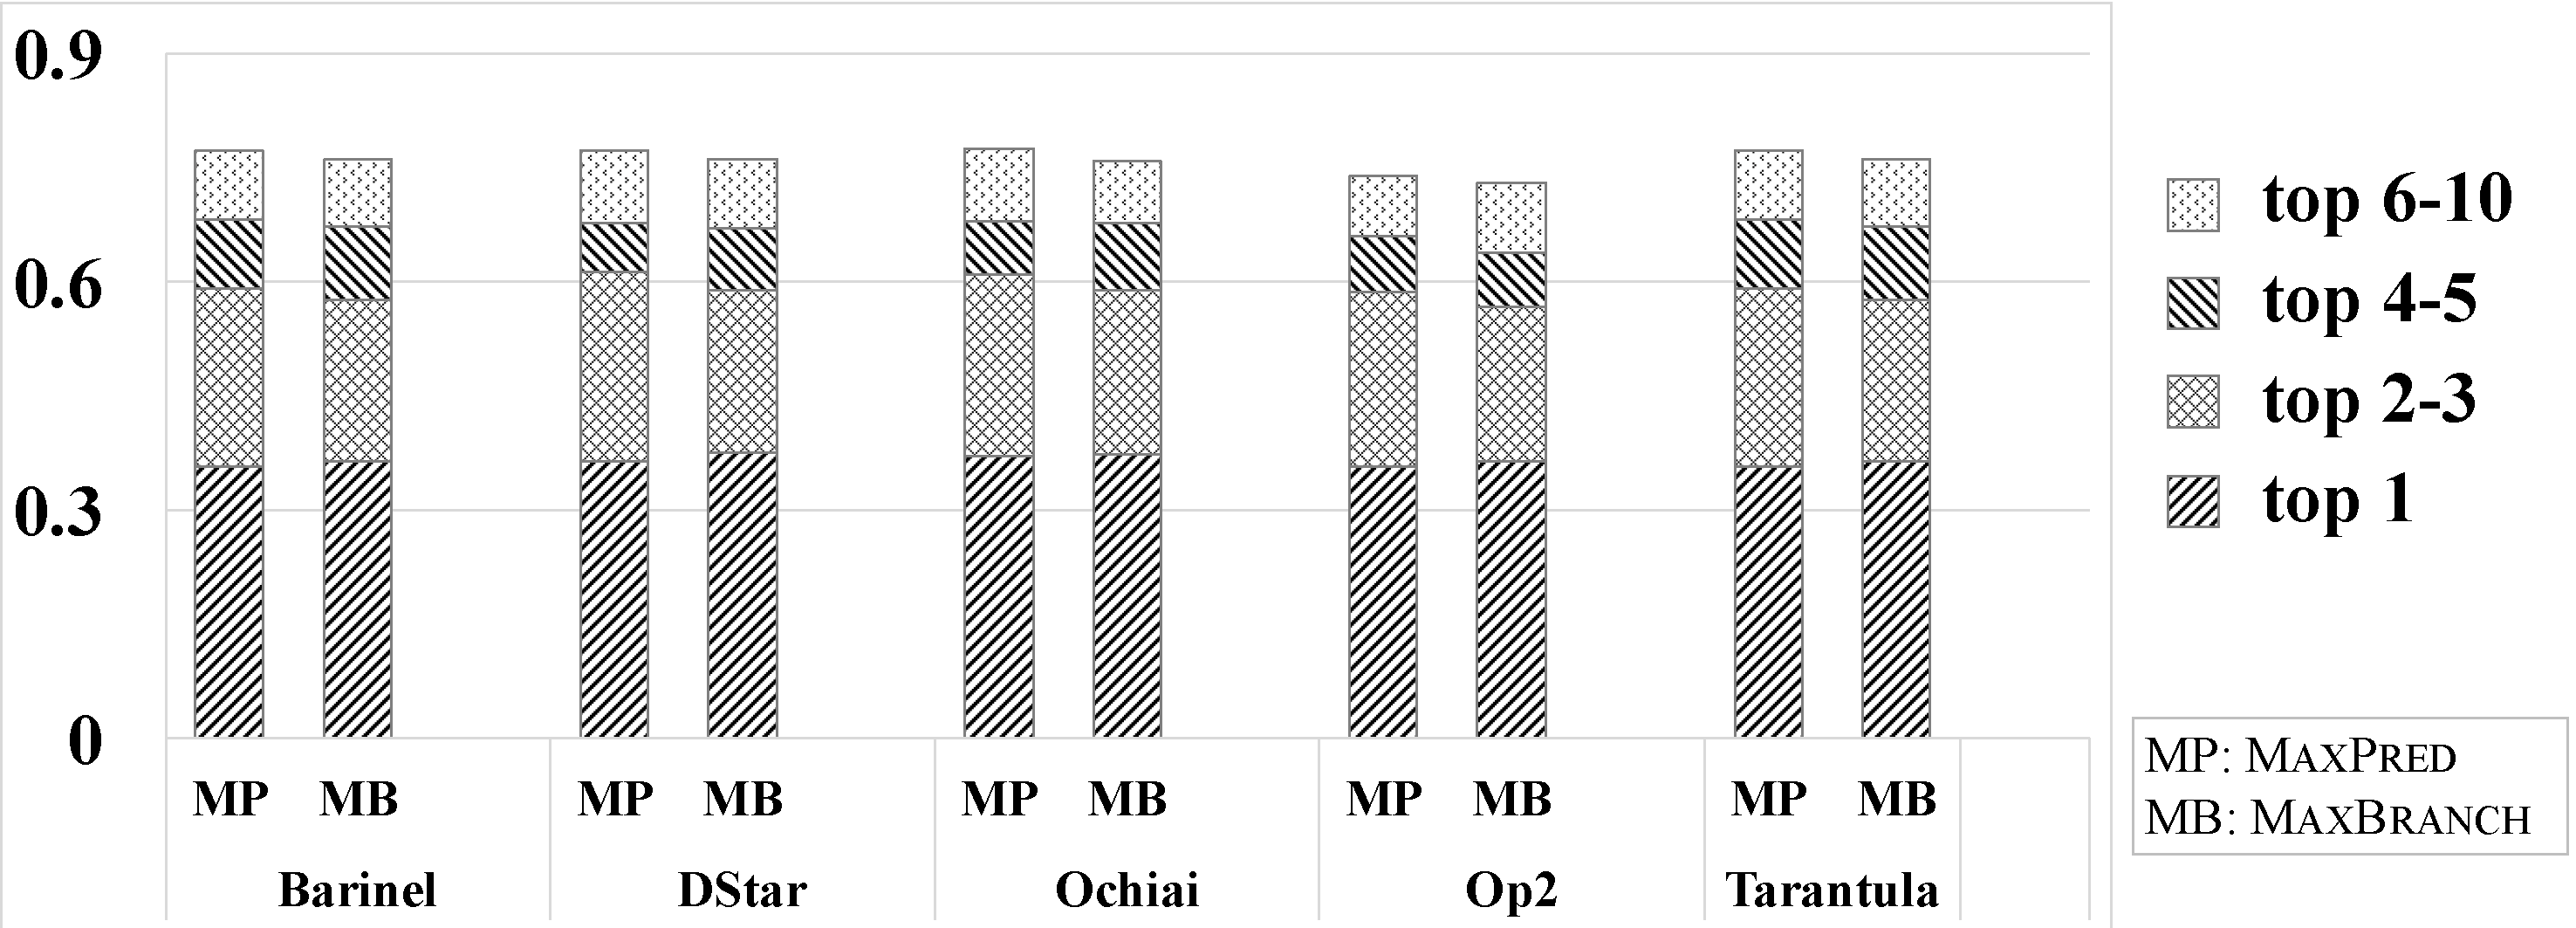
\includegraphics[width=16cm]{figure/branch-compare} 
\caption{分支谓词和全部预定义谓词的缺陷定位效果对比} 
\label{fig:branch-compare}
\end{figure}

\subsubsection{预测谓词}
\label{sec:eval_pref_predict}

对于预测出的谓词,进一步分析是怎样的谓词起了积极的作用。
对于程序元素$e$和它的谓词$P$,
谓词$P$被认为是对定位效果有积极的影响,如果$c_0 > c_1$且$e$是缺陷程序元素,或者$c_0 < c_1$且$e$不是缺陷程序元素。
其中$c_0$表示只使用神经网络或者随机森林谓词的结果\textsc{MaxDnn},
$c_1$表示基于频谱的缺陷定位的结果。

在所有 330 个项目中,神经网络有 511 个具有积极影响的谓词,随机森林模型有 1013 个具有积极影响的谓词。
这些具有积极影响的谓词具有多种表达形式。
部分高频出现的谓词类型如表\ref{top_predicate}所示。
百分比表示的是相对于积极影响谓词的百分比。
可见最起积极作用的谓词是对空指针的判断,然后是和零的比较。
这两种谓词加起来已经超过了积极谓词数量的50\%。
前面三种都是和常数的比较。
第四个“与极限值比较”表示的是与类似\mycode{Integer.MAX\_VALUE}这样的极限值进行比较。
虽然也是常数值,但是是和类型相关的常数值(\mycode{Integer.MAX\_VALUE, Double.MAX\_VALUE, Long.MAX\_VALUE, Double.MIN\_VALUE}都有出现),说明了类型特征的作用。
第五个是一个和变量\mycode{n}的比较。
这个比较有意思,说明虽然是不同项目的谓词,但是\mycode{n}这样的变量经常被用于边界值。
表明了开发者在开发时具有的某些通用的习惯。
第六个是和-1的比较,也是和常数的比较。

使用不同的机器学习模型,虽然预测数来的谓词数量有差别,
但是其谓词类型分布百分比非常相似。
两种模型最多的都是空指针判断。
而且可以发现,对于随机森林模型来说,空指针判断已经占到了积极谓词的接近40\%。
不过也有很多具有积极作用的谓词只出现了一两次,
这些谓词往往和上下文密切相关。

\begin{table}
\centering
\begin{tabular}{|l|r|r|r|r|r|r|}
\hline
\multirow{2}*{谓词类型} & \multicolumn{3}{c|}{神经网络模型} & \multicolumn{3}{c|}{随机森林模型} \\
\cline{2-7}
& 数量 & 百分比 & 累积百分比 & 数量 & 百分比 & 累积百分比 \\
\hline
空指针判断 & 155 & 30.33\% & 30.33\% & 400 & 39.49\% & 39.49\%\\
\hline
与0或0.0比较 & 125 & 24.46\% & 54.79\% & 222 & 21.92\% & 61.40\%\\
\hline
与1比较 & 34 & 6.65\% & 61.45\% & 58 & 5.73\% & 67.13\%\\
\hline
与极限值比较 & 32 & 6.65\% & 67.71\% & 30 & 2.96\% & 70.09\% \\
\hline
与\mycode{n}比较 & 18 & 3.52\% & 71.23\% & 11 & 1.09\% & 71.17\%\\
\hline
与-1比较 & 16 & 3.13\% & 74.36\% & 35 & 3.46\% & 74.63\%\\
\hline
\end{tabular}
\caption{预测出的产生积极影响的部分谓词}
\label{top_predicate}
\end{table}

\subsection{结合预定义谓词和预测谓词}

是否可以把预定义谓词和预测谓词结合呢?
回答是肯定的。
使用Top-1更高的神经网络模型\textsc{LinDnn}与\textsc{LinSD}结合。
使用的谓词为神经网络预测的谓词和预定义谓词的并集。
结果如表\ref{comb_pred_dnn}。
可以发现,Top-1指标上结合后相比于\textsc{LinSD}提升了5个缺陷。
总体上来说,结合后的效果比\textsc{LinSD}和\textsc{LinDnn}都要更好。
可见两种谓词在一定程度上具有互补性。

\finding{预测谓词与预定义谓词结合后效果进一步提升,二者具有互补性。}

\begin{table}
\centering
\begin{tabular}{|l|r|r|r|r|}
\hline
缺陷定位方法 & Top-1 & Top-3 & Top-5 & Top-10 \\
\hline
\textsc{LinSD} & 139 & 218 & 238 & 262 \\
\hline
\textsc{LinDnn} & 138 & 207 & 240 & 267 \\
\hline
\textsc{LinSD + LinDnn} & 144 &218 & 240 & 266 \\
\hline
\end{tabular}
\caption{预测谓词和预定义谓词的缺陷定位效果对比-具体数值}
\label{comb_pred_dnn}
\end{table}

% 一个谓词被认为是对定位效果有消极影响,如果$c_0 < c_1$且$e$是缺陷程序元素,或者$c_0 > c_1$且$e$不是缺陷程序元素。
% 于是谓词被分为两类(不满足以上两类的属于既没有积极影响,也没有消极影响的谓词),
% 这两类在不同的怀疑度计算公式下的分布情况如图\ref{fig:improve-deteriorate}。
% 可以发现大部分谓词还是对结果有积极影响的,只有少部分会对结果产生不好的影响。

